%% LyX 2.3.4.2 created this file.  For more info, see http://www.lyx.org/.
%% Do not edit unless you really know what you are doing.
\documentclass[english,dvipsnames,aspectratio=169,handout]{beamer}
\usepackage{mathptmx}
\usepackage{eulervm}
\usepackage[T1]{fontenc}
\usepackage[latin9]{inputenc}
\usepackage{babel}
\usepackage{amstext}
\usepackage{amssymb}
\usepackage{graphicx}
\usepackage{ifthen}
\usepackage{xcolor}
\usepackage{xspace}
\usepackage{tikz}
\usetikzlibrary{tikzmark}
\usetikzlibrary{calc}
\usepackage{pgfplots}
%\pgfplotsset{compat=1.17}
\usepackage{booktabs}
\usepackage{xpatch}
\usepackage{bbm}


\newcommand{\notenew}[1]{\note{#1}}

\xpatchcmd{\itemize}
  {\def\makelabel}
  {\ifnum\@itemdepth=1\relax
     \setlength\itemsep{2ex}% separation for first level
   \else
     \ifnum\@itemdepth=2\relax
       \setlength\itemsep{1ex}% separation for second level
     \else
       \ifnum\@itemdepth=3\relax
         \setlength\itemsep{0.5ex}% separation for third level
   \fi\fi\fi\def\makelabel
  }
 {}
 {}

\ifx\hypersetup\undefined
  \AtBeginDocument{%
    \hypersetup{unicode=true,pdfusetitle,
 bookmarks=true,bookmarksnumbered=false,bookmarksopen=false,
 breaklinks=false,pdfborder={0 0 0},pdfborderstyle={},backref=false,colorlinks=true,
 allcolors=NYUPurple,urlcolor=LightPurple}
  }
\else
  \hypersetup{unicode=true,pdfusetitle,
 bookmarks=true,bookmarksnumbered=false,bookmarksopen=false,
 breaklinks=false,pdfborder={0 0 0},pdfborderstyle={},backref=false,colorlinks=true,
 allcolors=NYUPurple,urlcolor=LightPurple}
\fi

\makeatletter

%%%%%%%%%%%%%%%%%%%%%%%%%%%%%% LyX specific LaTeX commands.
%% Because html converters don't know tabularnewline
\providecommand{\tabularnewline}{\\}

%%%%%%%%%%%%%%%%%%%%%%%%%%%%%% Textclass specific LaTeX commands.
% this default might be overridden by plain title style
\newcommand\makebeamertitle{\frame{\maketitle}}%
% (ERT) argument for the TOC
\AtBeginDocument{%
  \let\origtableofcontents=\tableofcontents
  \def\tableofcontents{\@ifnextchar[{\origtableofcontents}{\gobbletableofcontents}}
  \def\gobbletableofcontents#1{\origtableofcontents}
}

%%%%%%%%%%%%%%%%%%%%%%%%%%%%%% User specified LaTeX commands.
\usetheme{CambridgeUS} 
\beamertemplatenavigationsymbolsempty


% Set Color ==============================
\definecolor{NYUPurple}{RGB}{87,6,140}
\definecolor{LightPurple}{RGB}{165,11,255}


\setbeamercolor{title}{fg=NYUPurple}
\setbeamercolor{frametitle}{fg=NYUPurple}

\setbeamercolor{background canvas}{fg=NYUPurple, bg=white}
\setbeamercolor{background}{fg=black, bg=NYUPurple}

\setbeamercolor{palette primary}{fg=black, bg=gray!30!white}
\setbeamercolor{palette secondary}{fg=black, bg=gray!20!white}
\setbeamercolor{palette tertiary}{fg=gray!20!white, bg=NYUPurple}

\setbeamertemplate{headline}{}
\setbeamerfont{itemize/enumerate body}{}
\setbeamerfont{itemize/enumerate subbody}{size=\normalsize}
\setbeamerfont{itemize/enumerate subsubbody}{size=\normalsize}

\setbeamercolor{parttitle}{fg=NYUPurple}
\setbeamercolor{sectiontitle}{fg=NYUPurple}
\setbeamercolor{sectionname}{fg=NYUPurple}
\setbeamercolor{section page}{fg=NYUPurple}
%\setbeamercolor{description item}{fg=NYUPurple}
%\setbeamercolor{block title}{fg=NYUPurple}

\setbeamertemplate{blocks}[rounded][shadow=false]
\setbeamercolor{block body}{bg=normal text.bg!90!NYUPurple}
\setbeamercolor{block title}{bg=NYUPurple!30, fg=NYUPurple}



\AtBeginSection[]{
  \begin{frame}
  \vfill
  \centering
\setbeamercolor{section title}{fg=NYUPurple}
 \begin{beamercolorbox}[sep=8pt,center,shadow=true,rounded=true]{title}
    \usebeamerfont{title}\usebeamercolor[fg]{title}\insertsectionhead\par%
  \end{beamercolorbox}
  \vfill
  \end{frame}
}

\makeatother


\setlength{\parskip}{\medskipamount} 

\input ../macros

\begin{document}
\input ../rosenberg-macros


%\newtheorem{example}{Example}

\newcommand{\expect}{\mathbb{E}}
\newcommand{\variance}{\mathrm{Var}}
\DeclareMathOperator*{\Var}{Var}
\newcommand{\covariance}{\mathrm{Cov}}
\DeclareMathOperator*{\Cov}{Cov}
\newcommand{\prob}{\mathrm{Pr}}
\newcommand{\zeroVec}{\mathbf{0}}
\newcommand{\zeroMat}{\mathbf{0}}
\newcommand{\onesVec}{\mathbf{1}}
\newcommand{\ident}{\mathbf{I}}
\newcommand{\deriv}{\mathrm{d}}
\newcommand{\transpose}{\top}
\newcommand{\costDeriv}[1]{\overline{#1}}
\newcommand{\lossDeriv}{\costDeriv}
\newcommand{\normal}{\mathcal{N}}
\newcommand{\data}{\mathcal{D}}

\newcommand{\dataIdx}{i}
\newcommand{\featIdx}{j}
\newcommand{\dimIdx}{\featIdx}
\newcommand{\paramIdx}{\dimIdx}
\newcommand{\hidIdx}{i}
\newcommand{\classIdx}{k}
\newcommand{\outputIdx}{k}
\newcommand{\classIdxTwo}{\ell}
\newcommand{\featIdxTwo}{j^\prime}
\newcommand{\nfeat}{D}
\newcommand{\ndim}{\nfeat}
\newcommand{\ndata}{N}
\newcommand{\numClasses}{K}
\newcommand{\nout}{\numClasses}
\newcommand{\layerIdx}{\ell}
\newcommand{\numLayers}{L}
\newcommand{\nhid}{M}
\newcommand{\timeIdx}{t}
\newcommand{\ntime}{T}
\newcommand{\contextLen}{K}


\newcommand{\inputIJ}[2]{x^{(#1)}_{#2}}
\newcommand{\inputI}[1]{{\bf x}^{(#1)}}
\newcommand{\inputJ}[1]{x_{#1}}
\newcommand{\inputVec}{{\bf x}}
\newcommand{\inputVecT}[1]{\inputVec^{(#1)}}
\newcommand{\inputVecI}[1]{\inputVec^{(#1)}}
\newcommand{\inputUni}{x}
\newcommand{\inputUniI}[1]{x^{(#1)}}
\newcommand{\inputUniT}[1]{x^{(#1)}}
\newcommand{\inputMatrix}{\mathbf{X}}
\newcommand{\inputMatrixT}[1]{\inputMatrix^{(#1)}}
\newcommand{\targetI}[1]{t^{(#1)}}
\newcommand{\target}{t}
\newcommand{\targetK}[1]{\target_{#1}}
\newcommand{\targets}{\mathbf{t}}
\newcommand{\prediction}{y}
\newcommand{\predictionI}[1]{y^{(#1)}}
\newcommand{\predictionK}[1]{y_{#1}}
\newcommand{\predictionT}[1]{y^{(#1)}}
\newcommand{\predictions}{\mathbf{y}}
\newcommand{\predictionMatrix}{\mathbf{Y}}
\newcommand{\predictionMatrixT}[1]{\predictionMatrix^{(#1)}}
\newcommand{\intermediate}{z}
\newcommand{\intermediateI}[1]{\intermediate^{(#1)}}
\newcommand{\intermediateT}[1]{\intermediate^{(#1)}}
\newcommand{\intermediateK}[1]{\intermediate_{#1}}
\newcommand{\intermediates}{\mathbf{z}}
\newcommand{\intermediateMatrix}{\mathbf{Z}}
\newcommand{\intermediateMatrixT}[1]{\intermediateMatrix^{(#1)}}
\newcommand{\outIntermediate}{r}
\newcommand{\outIntermediateT}[1]{r^{(#1)}}
\newcommand{\outIntermediateK}[1]{\outIntermediate_{#1}}
\newcommand{\outIntermediates}{\mathbf{r}}
\newcommand{\outIntermediateMat}{\mathbf{R}}
\newcommand{\outIntermediateMatrix}{\mathbf{R}}
\newcommand{\outIntermediateMatrixT}[1]{\outIntermediateMatrix^{(#1)}}
\newcommand{\hiddenI}[1]{h_{#1}}
\newcommand{\hiddenT}[1]{h^{(#1)}}
\newcommand{\hiddenIT}[2]{h_{#1}^{(#2)}}
\newcommand{\hiddenLI}[2]{h_{#2}^{(#1)}}
\newcommand{\hiddens}{\mathbf{h}}
\newcommand{\hiddensL}[1]{\hiddens^{(#1)}}
\newcommand{\hiddensT}[1]{\hiddens^{(#1)}}
\newcommand{\hiddenMatrix}{\mathbf{H}}
\newcommand{\hiddenMat}{\hiddenMatrix}
\newcommand{\hiddenMatrixT}[1]{\hiddenMatrix^{(#1)}}
\newcommand{\hiddenMatL}[1]{\hiddenMat^{(#1)}}
\newcommand{\weights}{{\bf w}}
\newcommand{\weightsL}[1]{\weights^{(#1)}}
\newcommand{\weightJ}[1]{w_{#1}}
\newcommand{\weightLIJ}[3]{w^{(#1)}_{#2 #3}}
\newcommand{\weightLKI}[3]{w^{(#1)}_{#2 #3}}
\newcommand{\weightLJ}[2]{w^{(#1)}_{#2}}
\newcommand{\weightKJ}[2]{w_{#1 #2}}
\newcommand{\weightIJ}{\weightKJ}
\newcommand{\weightUni}{w}
\newcommand{\weightMat}{\mathbf{W}}
\newcommand{\weightMatL}[1]{\weightMat^{(#1)}}
\newcommand{\bias}{b}
\newcommand{\biasLI}[2]{\bias^{(#1)}_{#2}}
\newcommand{\biasLK}{\biasLI}
\newcommand{\biasL}[1]{\bias^{(#1)}}
\newcommand{\biasK}[1]{\bias_{#1}}
\newcommand{\biasJ}[1]{\bias_{#1}}
\newcommand{\biases}{\mathbf{b}}
\newcommand{\biasesL}[1]{\biases^{(#1)}}
\newcommand{\threshold}{r}
\newcommand{\featureJ}[1]{\psi_{#1}}
\newcommand{\featureVec}{{\boldsymbol \psi}}
\newcommand{\loss}{\mathcal{L}}
\newcommand{\lossI}[1]{\loss^{(#1)}}
\newcommand{\zeroOneLoss}{\loss_{\rm 0-1}}
\newcommand{\squaredErrorLoss}{\loss_{\rm SE}}
\newcommand{\crossEntropyLoss}{\loss_{\rm CE}}
\newcommand{\logisticCrossEntropyLoss}{\loss_{\rm LCE}}
\newcommand{\softmaxCrossEntropyLoss}{\loss_{\rm SCE}}
\newcommand{\hingeLoss}{\loss_{\rm H}}
\newcommand{\cost}{\mathcal{J}}
\newcommand{\regularizer}{\mathcal{R}}
\newcommand{\lrate}{\alpha}
\newcommand{\learningRate}{\lrate}
\newcommand{\featureMap}{{\boldsymbol \psi}}
\newcommand{\featureMapJ}[1]{\psi_{#1}}
\newcommand{\sigmoid}{\sigma}
\newcommand{\logistic}{\sigmoid}
\newcommand{\activationFunction}{\phi}
\newcommand{\activationFunctionL}[1]{\activationFunction^{(#1)}}
\newcommand{\activationFunctionTwo}{\psi}
\newcommand{\parityFunction}{f_{\rm par}}
\newcommand{\function}{f}
\newcommand{\functionL}[1]{\function^{(#1)}}
\newcommand{\indicatorOf}[1]{\mathbbm{1}_{#1}}
\newcommand{\softmax}{\mathrm{softmax}}
\newcommand{\weightCost}{\lambda}
\newcommand{\genCost}{\mathcal{C}}
\newcommand{\momentumVec}{\mathbf{p}}
\newcommand{\momentumJ}[1]{p_{#1}}
\newcommand{\momentumParam}{\mu}
\newcommand{\genParams}{{\boldsymbol \theta}}
\newcommand{\genParamJ}[1]{\theta_{#1}}
\newcommand{\pData}{p_{\mathcal{D}}}
\newcommand{\bestPrediction}{\prediction_\star}

\newcommand{\obs}{\mathbf{x}}
\newcommand{\obsJ}[1]{x_{#1}}
\newcommand{\obsI}[1]{\obs^{(#1)}}
\newcommand{\pfn}{\mathcal{Z}}
\newcommand{\happiness}{H}
\newcommand{\latents}{\mathbf{z}}

\newcommand{\state}{\mathbf{s}}
\newcommand{\stateT}[1]{\state_{#1}}
\newcommand{\act}{\mathbf{a}}
\newcommand{\actT}[1]{\act_{#1}}
\newcommand{\reward}{r}
\newcommand{\policy}{\pi}
\newcommand{\policyParams}{\boldsymbol{\theta}}
\newcommand{\policyTh}{{\policy_{\policyParams}}}
\newcommand{\MDP}{\mathcal{M}}
\newcommand{\rollout}{\tau}
\newcommand{\expectedReturn}{R}

\newcommand{\discReturn}{G}
\newcommand{\discFactor}{\gamma}
\newcommand{\valueFunc}{V}
\newcommand{\valueFuncPi}{\valueFunc^{\policy}}
\newcommand{\valueFuncPiTh}{\valueFunc^{\policyTh}}
\newcommand{\qFunc}{Q}
\newcommand{\qFuncPi}{\qFunc^{\policy}}
\newcommand{\optPolicy}{\policy^*}
\newcommand{\optQ}{\qFunc^*}

\newcommand{\subspace}{\mathcal{S}}
\newcommand{\projectedInput}{\tilde{\inputVec}}
\newcommand{\projectedInputI}[1]{\projectedInput^{(#1)}}
\newcommand{\codeVec}{\mathbf{z}}
\newcommand{\codeVecI}[1]{\codeVec^{(#1)}}
\newcommand{\dataMean}{\boldsymbol{\mu}}
\newcommand{\dataCov}{\boldsymbol{\Sigma}}
\newcommand{\pcaVec}{\mathbf{u}}

\newcommand{\featureMatrix}{{\boldsymbol \Psi}}
\newcommand{\smootherMatrix}{{\boldsymbol \Omega}}
\newcommand{\smootherMatrixEntry}{\Omega}
\newcommand{\hypothesis}{\mathcal{H}}
\newcommand{\priorMean}{\mathbf{m}}
\newcommand{\priorCov}{\mathbf{S}}
\newcommand{\priorVar}{\eta}
\newcommand{\postMean}{\boldsymbol{\mu}}
\newcommand{\postCov}{\boldsymbol{\Sigma}}
\newcommand{\predMean}{\mu_{\rm pred}}
\newcommand{\predVar}{\sigma^2_{\rm pred}}
\newcommand{\predStd}{\sigma_{\rm pred}}


\newcommand{\given}{\,|\,}
\newcommand{\TODO}[1]{{\color{red} {\bf [[#1]]}}}
\newcommand{\high}[1]{{\color{blue}{#1}}}



\newcommand{\naive}{na{\"\i}ve }































\title[CSCI-GA 2565]{Neural Networks II}
\author{Mengye Ren}

\date{September 26, 2023}
\institute{NYU}

\makebeamertitle
\mode<article>{Just in article version}


% \begin{frame}
% \begin{center}
% {\Huge CNN Interpretability}
% \end{center}
% \end{frame}

\section{Neural Networks Interpretability}

\begin{frame}{ML=Blackbox?}
\begin{center}
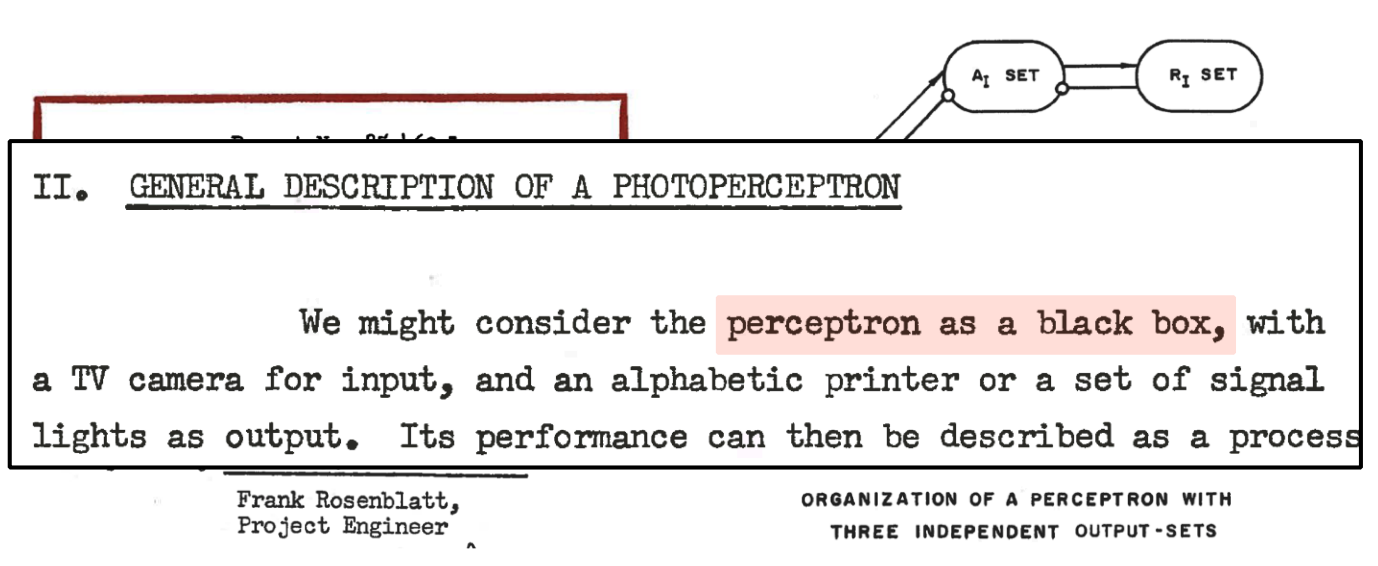
\includegraphics[width=\textwidth]{figures/blackbox.png}
\footnote{Slide credit: Wojciech Samek}
\end{center}

\end{frame}

\begin{frame}{ML Interpretability}
\begin{itemize}
  \item Linear regression: Weights represent feature selection strength
  \item SVMs: Dual weights represent sample selection
  \item Bayesian methods: Model the generative process as a probabilistic model, fully transparent
  \item Decision trees: If-else decision making process
  \item Neural networks: ?
\end{itemize}
\end{frame}

\begin{frame}{Feature Visualization}
\begin{itemize}
  \item Recall: we can understand what first-layer features are doing by visualizing the weight matrices.
  \item Higher-level weight matrices are hard to interpret.
  \begin{center}
    \begin{columns}
      \begin{column}{0.35 \textwidth}
        \begin{center}
          Fully connected
          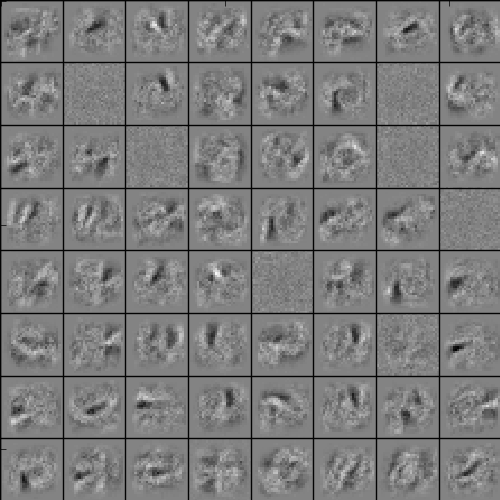
\includegraphics[width=0.6 \textwidth]{figures/mnist_filters.png}
        \end{center}
      \end{column}
      \begin{column}{0.35 \textwidth}
        \begin{center}
          Convolutional
          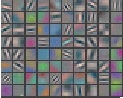
\includegraphics[width=0.55 \textwidth]{figures/zeiler_filters.pdf}
        \end{center}
        \begin{flushright}
  \tiny{Zeiler and Fergus, Visualizing and understanding convolutional networks, ECCV 2014.}
        \end{flushright}
      \end{column}
    \end{columns}
  \end{center}
\item The better the input matches these weights, the more the feature activates.
  \begin{itemize}
  \item Obvious generalization: visualize higher-level features by seeing what inputs activate them.
  \end{itemize}
\end{itemize}
\end{frame}

\begin{frame}{Feature Visualization}
\begin{itemize}
\item One way to formalize: pick the images in the training set which activate a unit most strongly.
\item Here's the visualization for layer 1:
  \begin{center}
    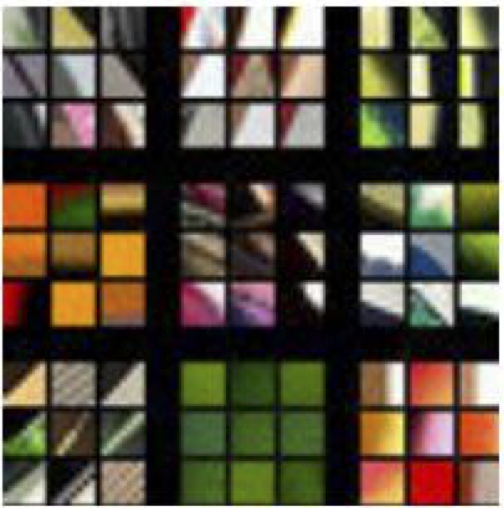
\includegraphics[width=0.3 \textwidth]{figures/layer1.png}
  \end{center}
\end{itemize}
\begin{flushright}
  \tiny{Zeiler and Fergus, Visualizing and understanding convolutional networks, ECCV 2014.}
\end{flushright}
\end{frame}

\begin{frame}{Feature Visualization}
\begin{itemize}
\item Layer 3:
  \begin{center}
    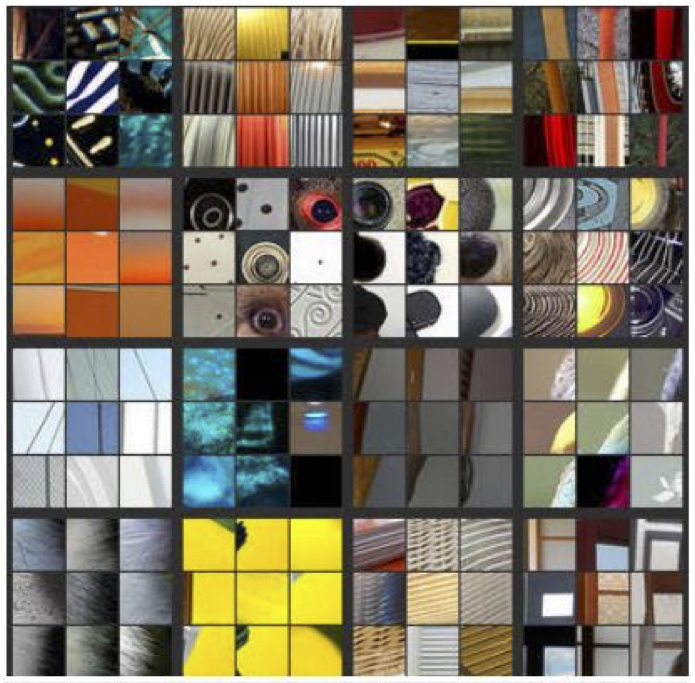
\includegraphics[width=0.4 \textwidth]{figures/layer3.png}
  \end{center}
\end{itemize}
\begin{flushright}
  \tiny{Zeiler and Fergus, Visualizing and understanding convolutional networks, ECCV 2014.}
\end{flushright}
\end{frame}

\begin{frame}{Feature Visualization}
\begin{itemize}
\item Layer 4:
  \begin{center}
    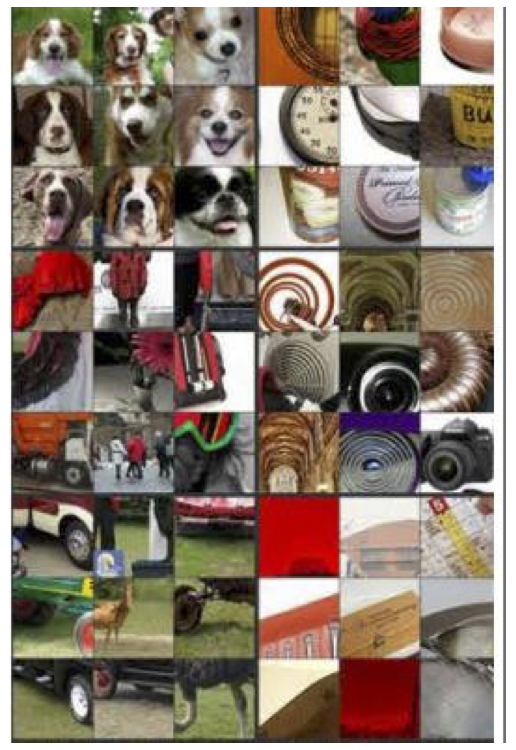
\includegraphics[width=0.4 \textwidth]{figures/layer4.png}
  \end{center}
\end{itemize}
\begin{flushright}
  \tiny{Zeiler and Fergus, Visualizing and understanding convolutional networks, ECCV 2014.}
\end{flushright}
\end{frame}

\begin{frame}{Feature Visualization}
\begin{itemize}
\item Layer 5:
  \begin{center}
    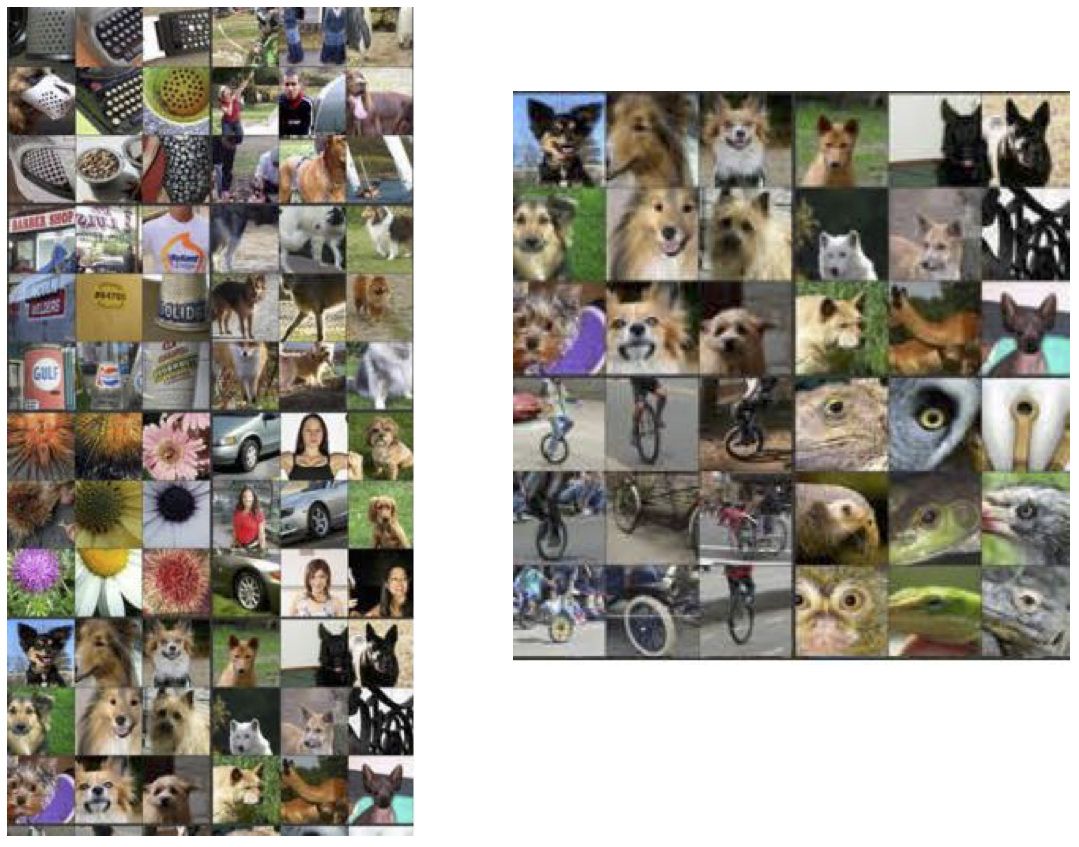
\includegraphics[width=0.7 \textwidth]{figures/layer5.png}
  \end{center}
\end{itemize}
\begin{flushright}
  \tiny{Zeiler and Fergus, Visualizing and understanding convolutional networks, ECCV 2014.}
\end{flushright}
\end{frame}

\begin{frame}{Feature Visualization}
\begin{itemize}
  \item Higher layers seem to pick up more abstract, high-level information.
  \item Problems?
    \begin{itemize}
    \item Can't tell what the unit is actually responding to in the image.
    \item We may read too much into the results, e.g.~a unit may detect red, and the images that maximize its activation will all be stop signs.
    \end{itemize}
  \item Can use input gradients to diagnose what the unit is responding to.
\end{itemize}
\end{frame}

\begin{frame}{Feature Visualization}
\begin{itemize}
\item Input gradients can be hard to interpret.
\item Take a good object recognition conv net (Alex Net) and compute the gradient of $\log p(y= \textrm{``cat''} | \inputVec)$:
  \begin{center}
    \begin{columns}
      \begin{column}{0.35 \textwidth}
        \begin{center}
          Original image
          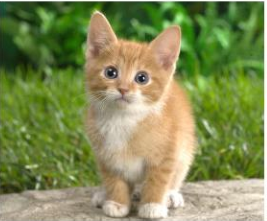
\includegraphics[width=0.8 \textwidth]{figures/cat.pdf}
        \end{center}
      \end{column}
      \begin{column}{0.35 \textwidth}
        \begin{center}
          Gradient for ``cat''
          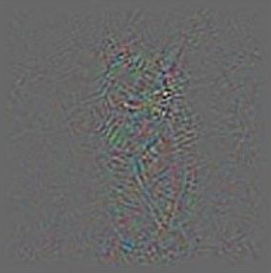
\includegraphics[width=0.7 \textwidth]{figures/cat_gradient.pdf}
        \end{center}
      \end{column}
    \end{columns}
  \end{center}
\end{itemize}
\end{frame}

\begin{frame}{Feature Visualization}
  \begin{itemize}
  \item \high{Guided backprop} is a total hack to prevent this cancellation.
  \item Do the backward pass as normal, but apply the ReLU nonlinearity to all the activation error signals.
    \[ y = \textrm{ReLU}(z) \qquad \bar{z} = \begin{cases} \bar{y} & \text{if $z > 0$ {\color{red} and $\bar{y} > 0$}} \\ 0 & \text{otherwise} \end{cases} \]
  \item We want to visualize what excites given unit, not what suppresses it.
    \begin{center}
      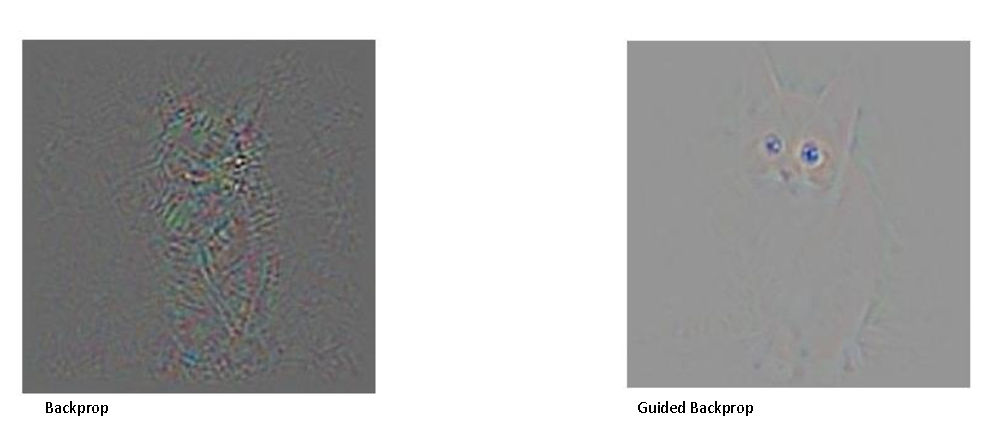
\includegraphics[width=0.5 \textwidth]{figures/guided_backprop_results.pdf}
    \end{center}
  \end{itemize}
\end{frame}

\begin{frame}{Guided Backprop}
\begin{center}
  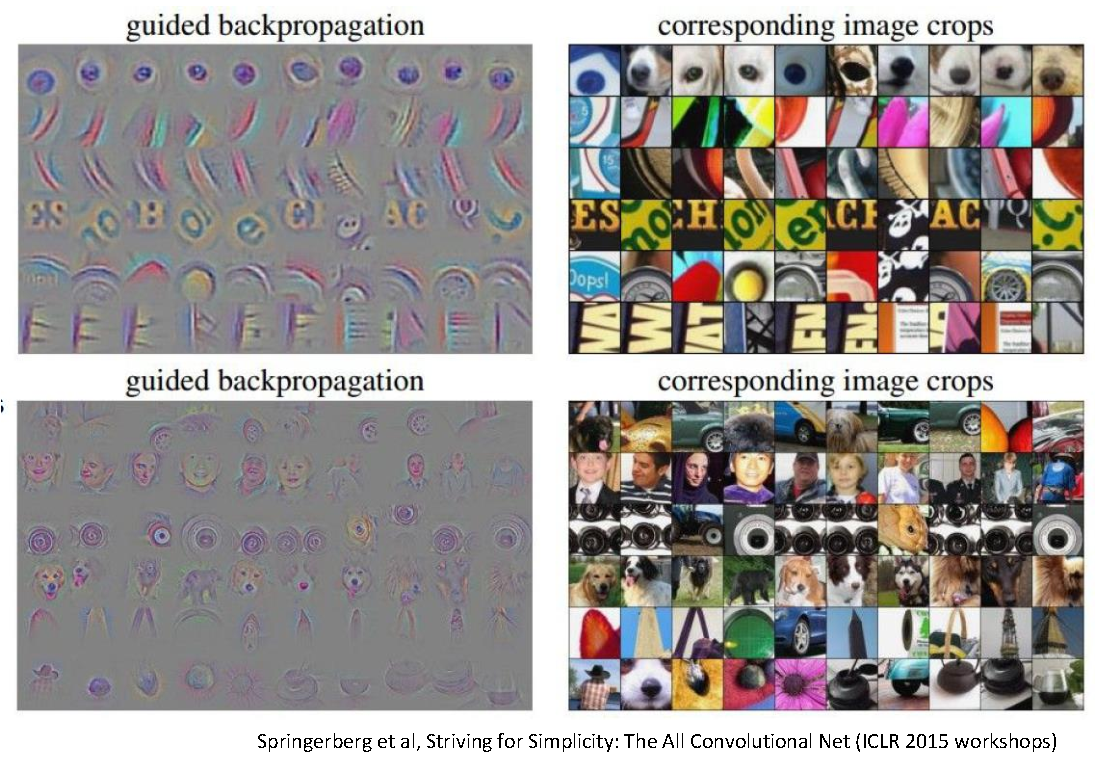
\includegraphics[width=0.85 \textwidth]{figures/guided_backprop_results2.pdf}
\end{center}
\begin{flushright}
{\tiny Springerberg et al., Striving for simplicity: The all convolutional net, ICLR workshop 2015.}
\end{flushright}

\notenew{
\begin{itemize}
  \item We start from here.
  \item Visualize one neuron in the input image.
  \item Draw one neuron in the middle.
\end{itemize}
}
\end{frame}


\begin{frame}{Class activation map (CAM)}

Classification networks typically use global avg pooling before the final layer.

This pooling layer can already contain semantic information.

We can visualize a heat map 

\begin{center}
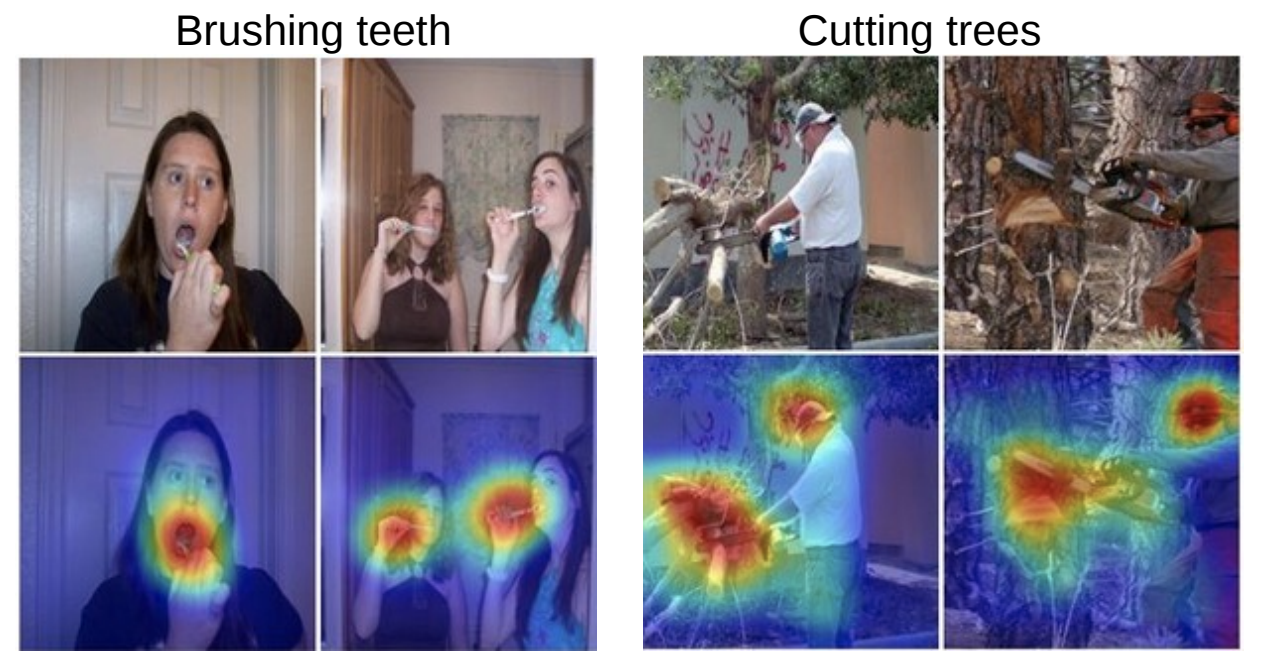
\includegraphics[height=0.3\textheight]{figures/cam.png}
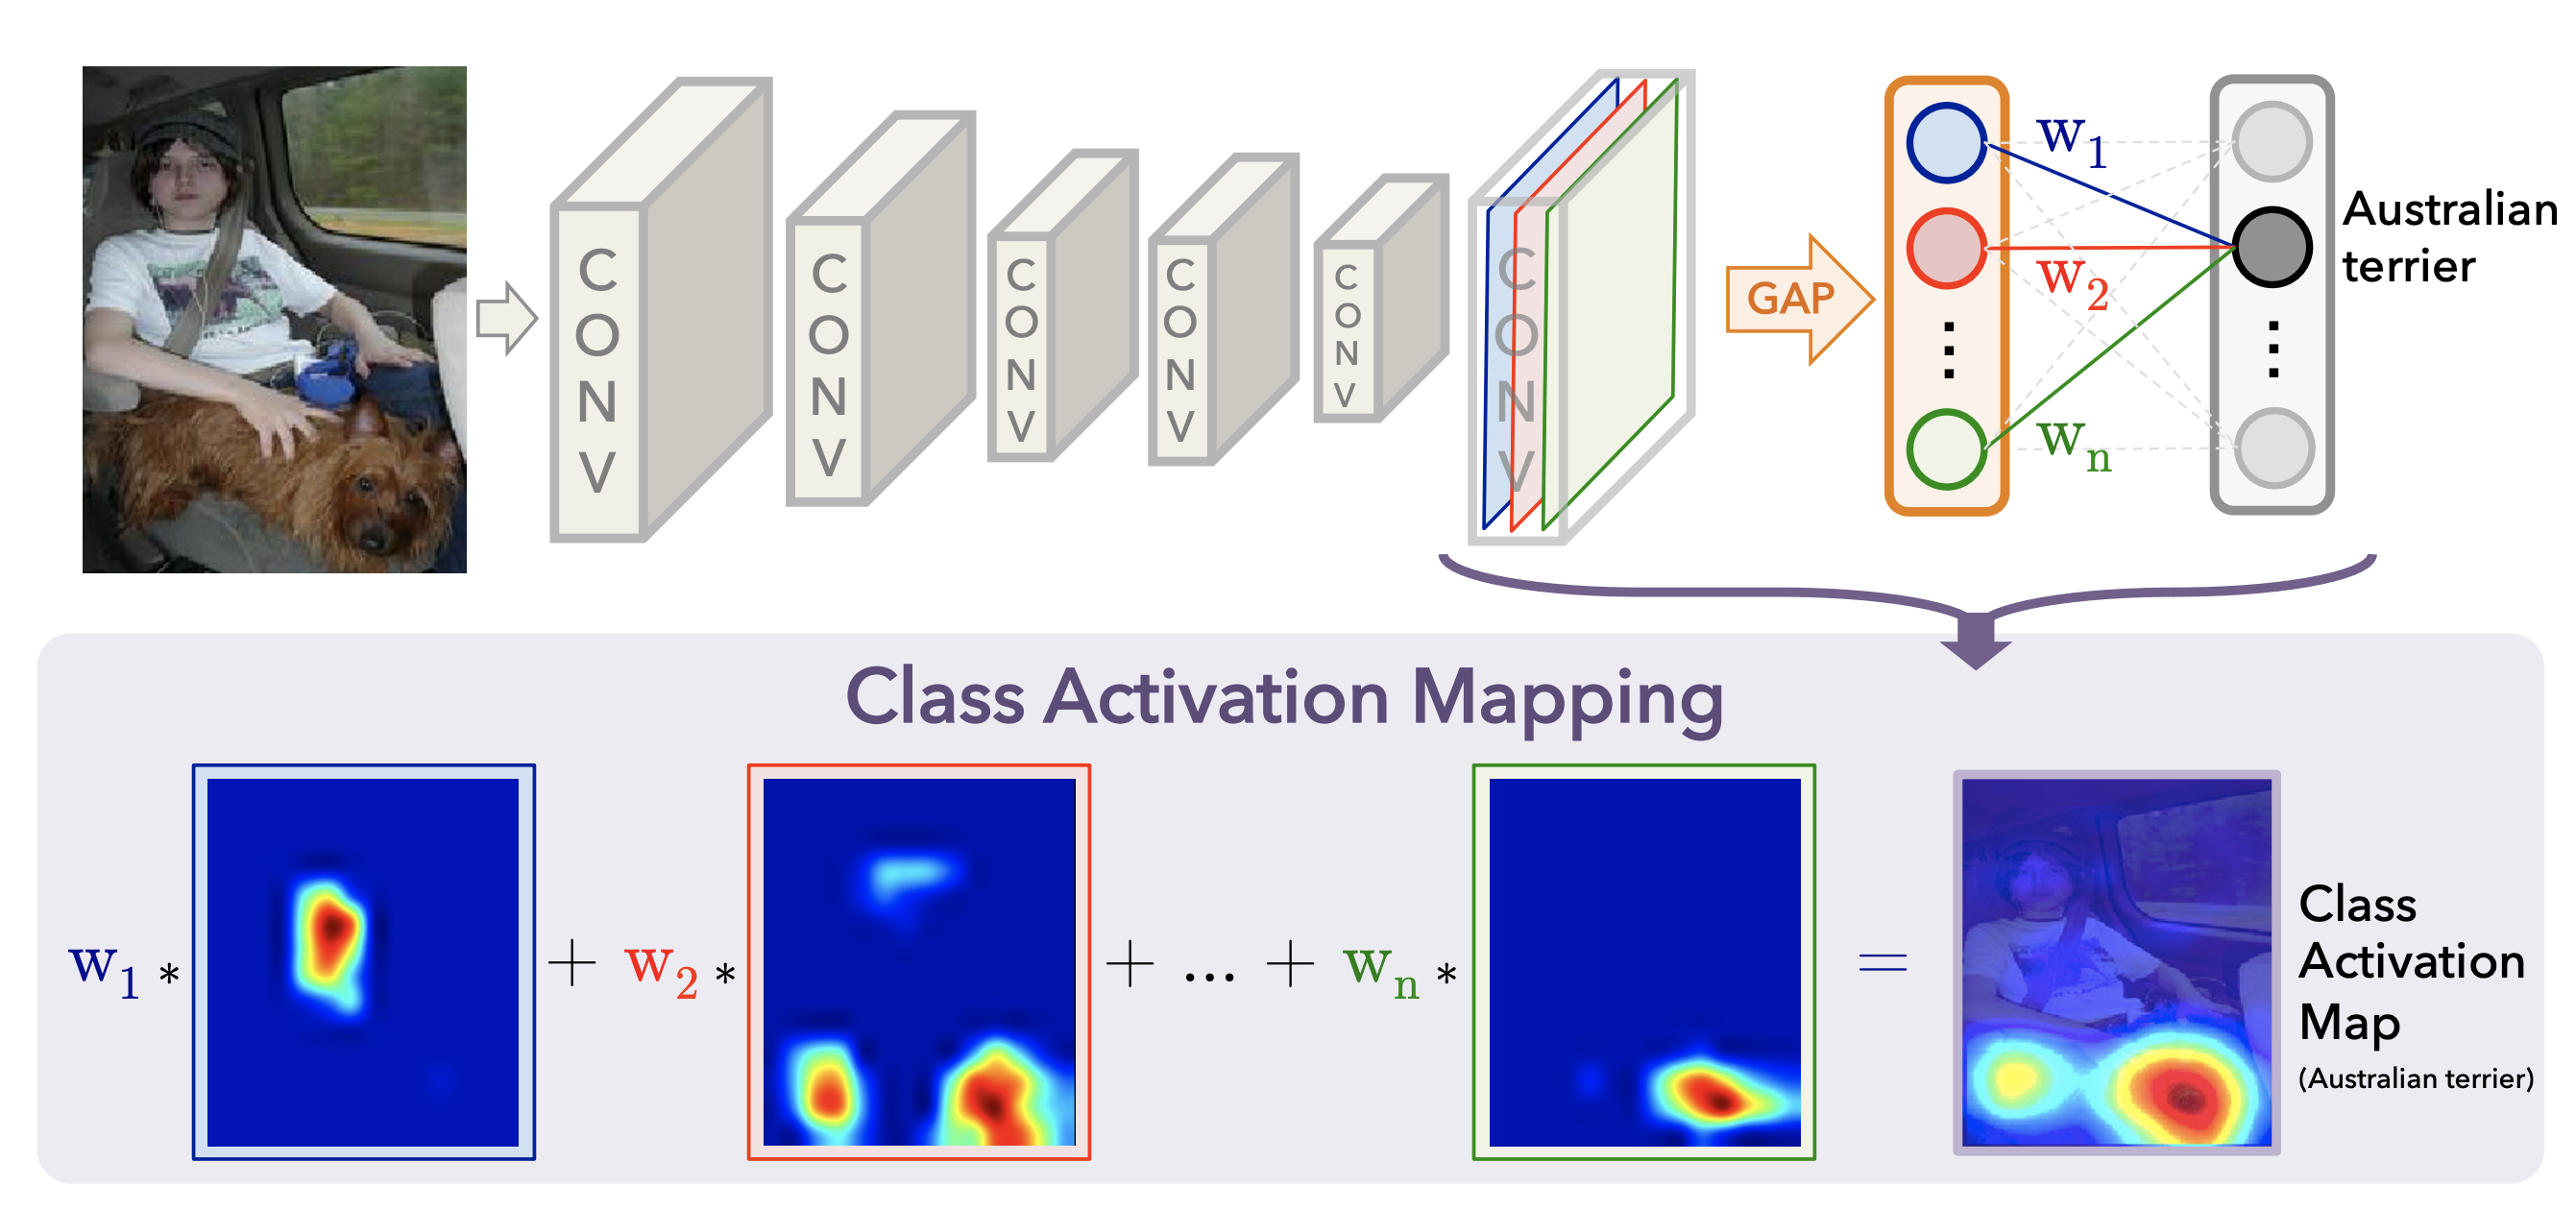
\includegraphics[height=0.3\textheight]{figures/cam2.png}
\end{center}

\begin{flushright}
{\tiny Zhou et al. Learning deep features for discriminative localization. CVPR 2016.}
\end{flushright}

\notenew{
  \begin{itemize}
    \item Another way is to think about the output classes.
    \item Imagine you have a classifier.
    \item What would be the region of the input that is responsible 
    \item Utilize the average pooling layer.
    \item Take the dot product between the activation at each location and the class vector
  \end{itemize}
}
\end{frame}

\begin{frame}{GradCAM}

\begin{center}
\vspace{-0.2in}
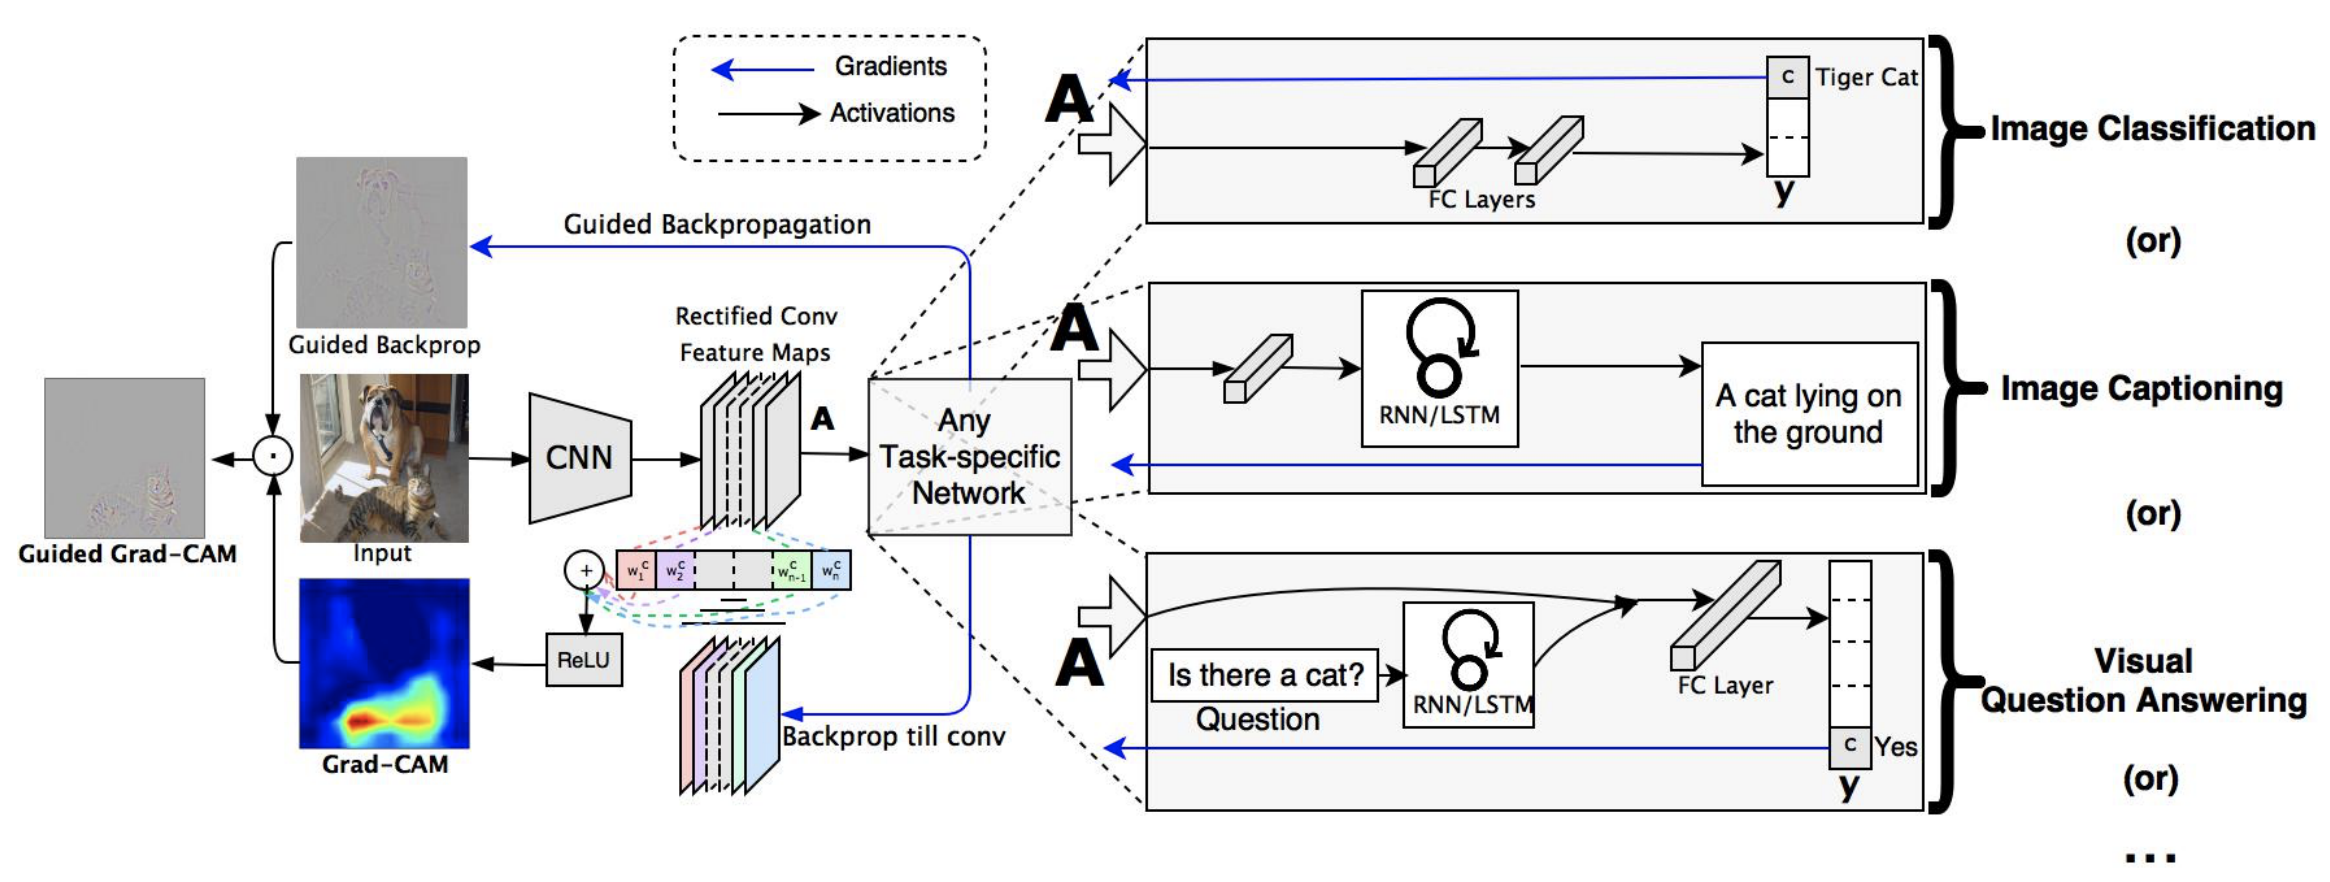
\includegraphics[width=0.7\textwidth]{figures/gradcam.png}
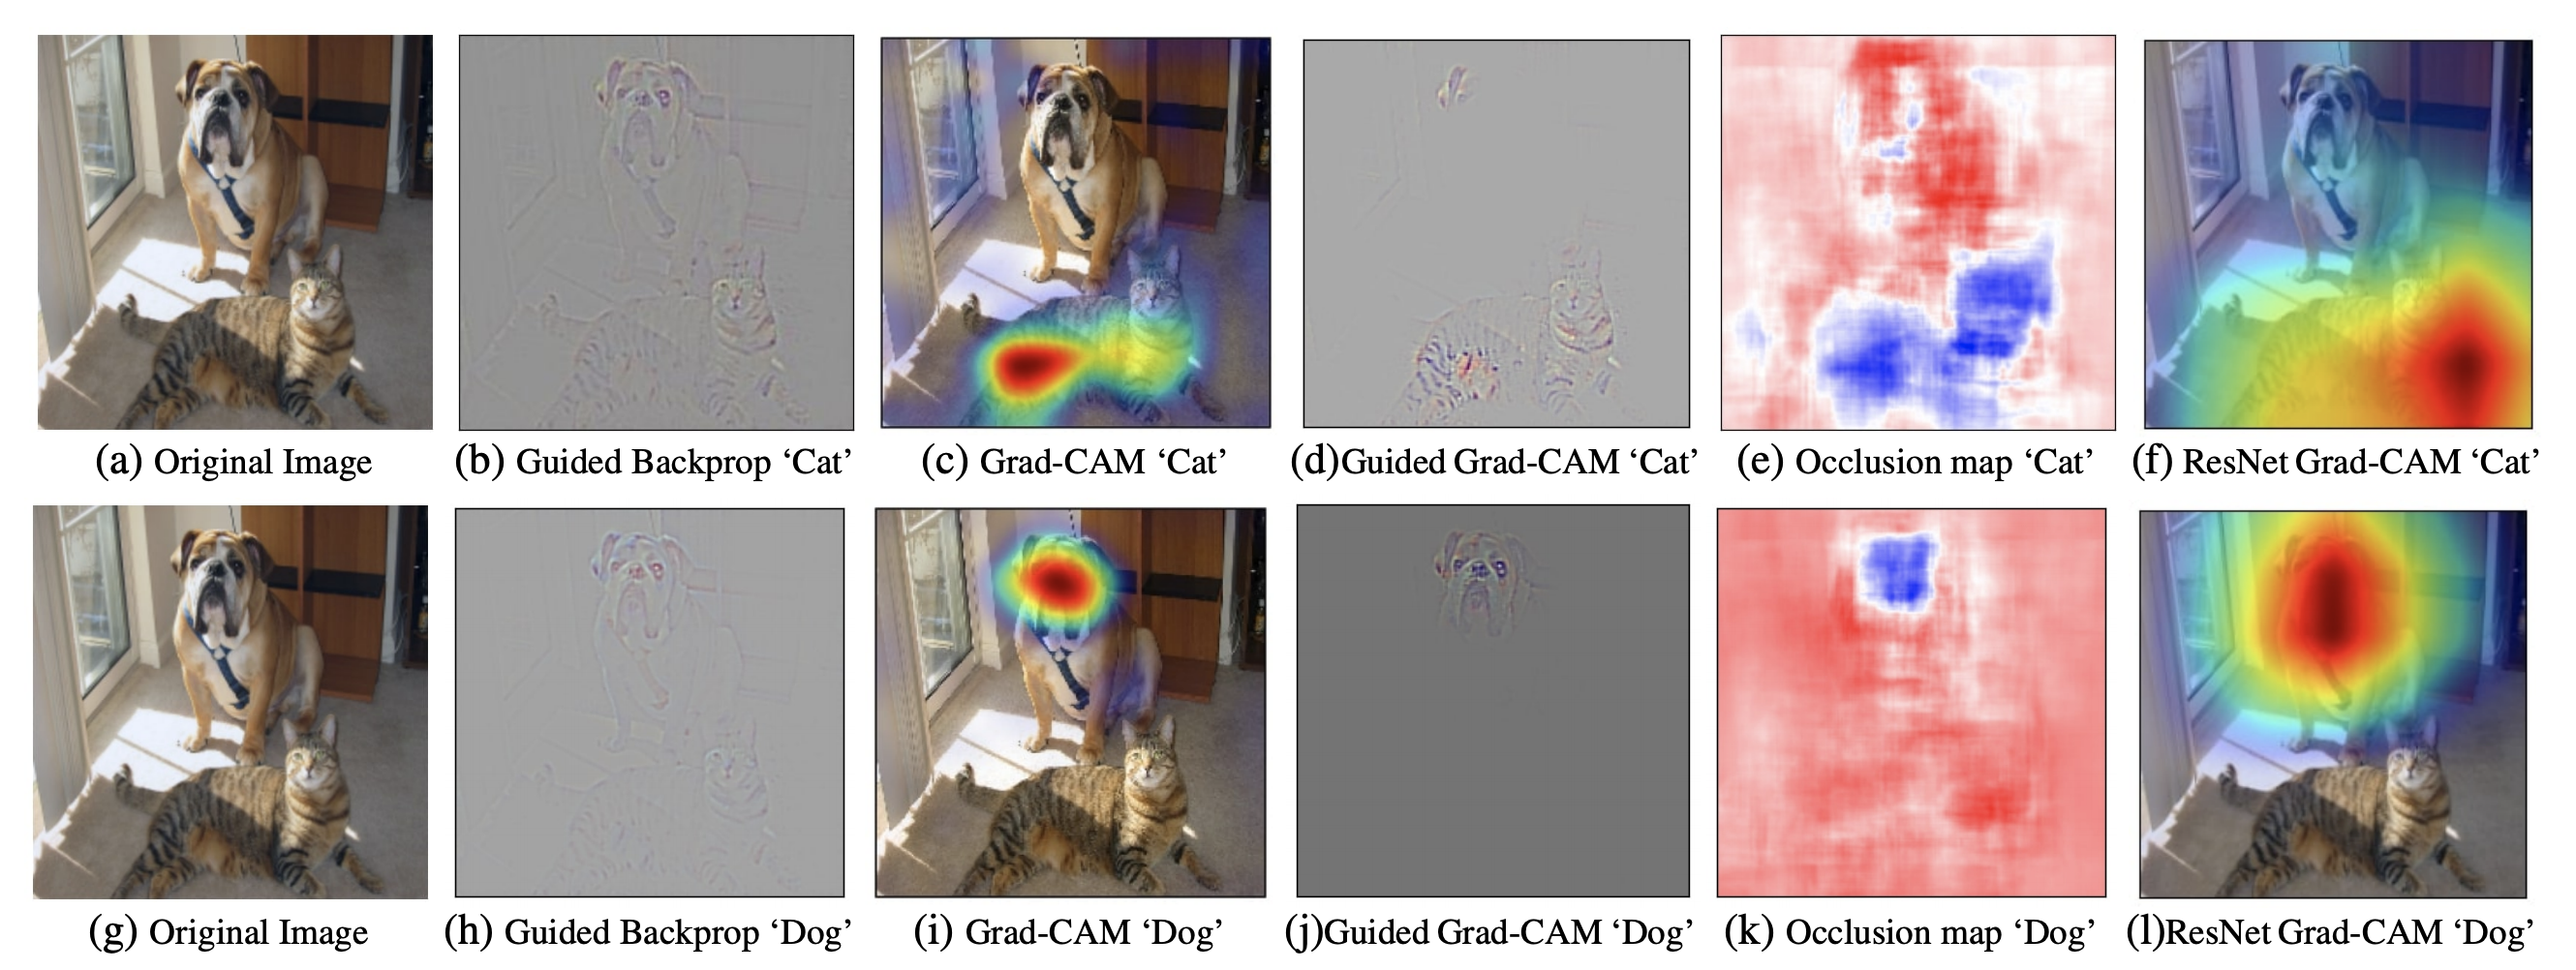
\includegraphics[width=0.45\textwidth,trim={0 0 16cm 0},clip]{figures/gradcam2.png}
\end{center}

\begin{flushright}
{\tiny Selvaraju et al. Grad-CAM: Visual explanations from deep networks via gradient-based localization. ICCV 2017.}
\end{flushright}

\notenew{
  \begin{itemize}
    \item Potentially a way to combine guided backprop and CAM.
    \item In the example, GBP is still plotting the dog, even though we are visualizing the cat neuron.
    \item We can suppress it by overlapping it with CAM.
  \end{itemize}
}
\end{frame}

\begin{frame}{Gradient Ascent on Images}
\begin{itemize}
\item Can do gradient ascent on an image to maximize the activation of a given neuron.
  \begin{center}
    \hspace{-3em}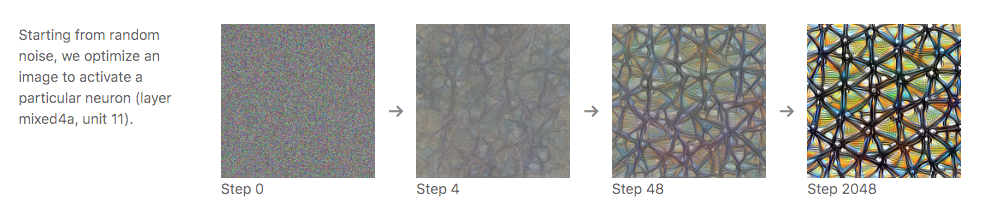
\includegraphics[width=\textwidth]{figures/distill_gd.png}
  \end{center}
\end{itemize}
\begin{flushright}
  \begin{tiny}
    \vspace{-1em}
    \url{https://distill.pub/2017/feature-visualization/}
  \end{tiny}
\end{flushright}

\notenew{
  \begin{itemize}
    \item Guided backpropagation = 1 step
    \item What if we run multiple steps of gradients?
  \end{itemize}
}
\end{frame}

\begin{frame}{Gradient Ascent on Images}
\begin{center}
  \hspace{-1em}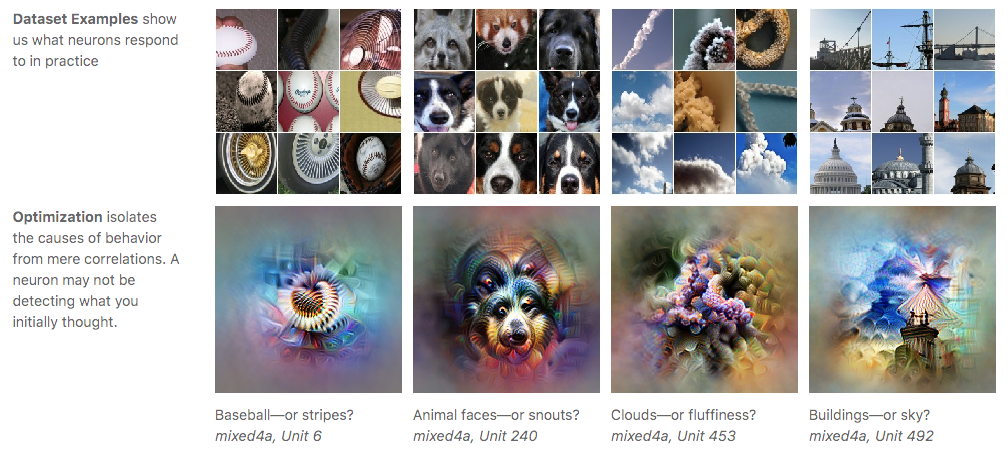
\includegraphics[width=\textwidth]{figures/distill_why_optimize.png}
\end{center}
\begin{flushright}
  \begin{tiny}
    \vspace{-1em}
    \url{https://distill.pub/2017/feature-visualization/}
  \end{tiny}
\end{flushright}

\notenew{
  \begin{itemize}
    \item For the same layer, we can run it on different units, and get different results.
    \item Above: dataset examples that maximizes neuron activation
    \item Below: optimized images that maximizes neuron activation
  \end{itemize}
}
\end{frame}

\begin{frame}{Gradient Ascent on Images}
\begin{itemize}
  \item Higher layers in the network often learn higher-level, more interpretable representations
    \begin{center}
      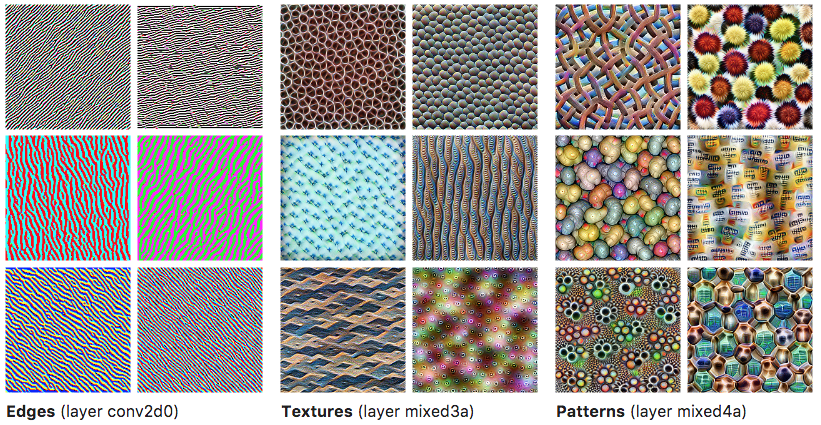
\includegraphics[width=0.85 \linewidth]{figures/olah.png}
    \end{center}
    \begin{flushright}
      \begin{tiny}
        \vspace{-1em}
        \url{https://distill.pub/2017/feature-visualization/}
      \end{tiny}
    \end{flushright}
\end{itemize}
\end{frame}

\begin{frame}{Gradient Ascent on Images}
\begin{itemize}
  \item Higher layers in the network often learn higher-level, more interpretable representations
    \begin{center}
      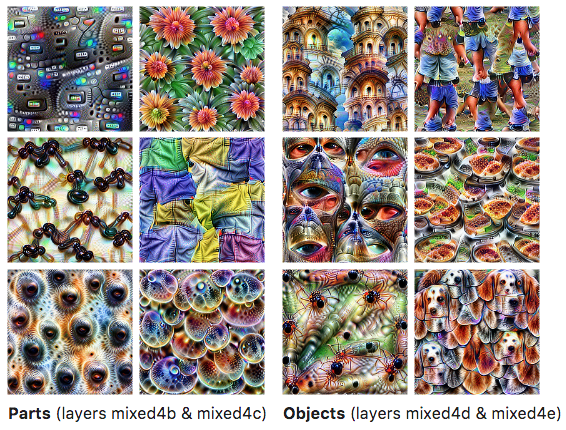
\includegraphics[width=0.6 \linewidth]{figures/olah2.png}
    \end{center}
    \begin{flushright}
      \begin{tiny}
        \vspace{-1em}
        \url{https://distill.pub/2017/feature-visualization/}
      \end{tiny}
    \end{flushright}
\end{itemize}
\end{frame}

\begin{frame}{Deep dream}
\begin{itemize}
\item Start with an image, and run a conv net on it.
\item Change the image such that units which were already highly activated get activated even more strongly.
``Rich get richer.''
\end{itemize}
\begin{center}
  \hspace{-1em}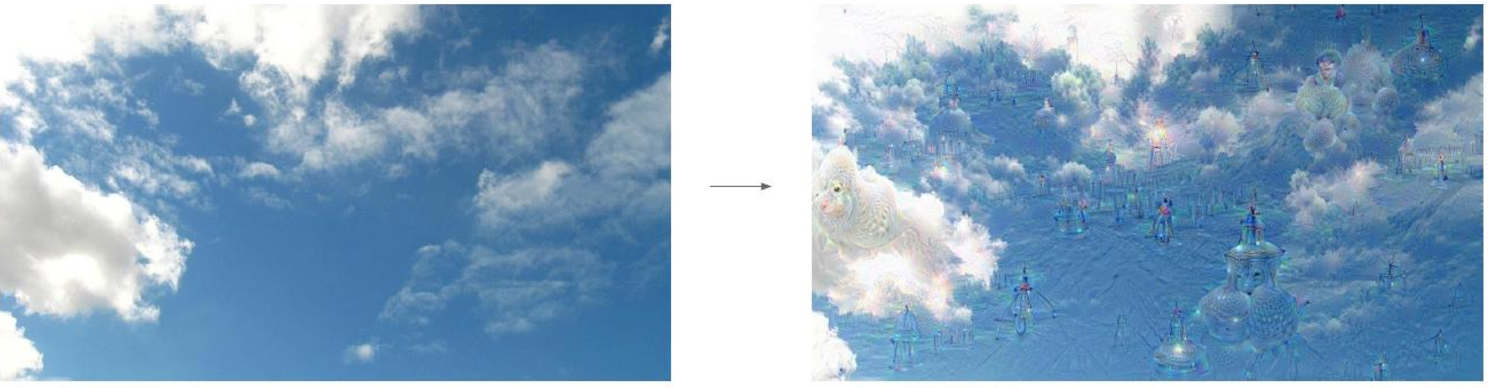
\includegraphics[width=\textwidth]{figures/deepdream1.pdf}
\end{center}

\notenew{
\begin{itemize}
  \item What if we try to maximize all neuron in one layer at once?
\end{itemize}
}
\end{frame}

\begin{frame}{Deep dream}
\begin{center}
  \hspace{-1em}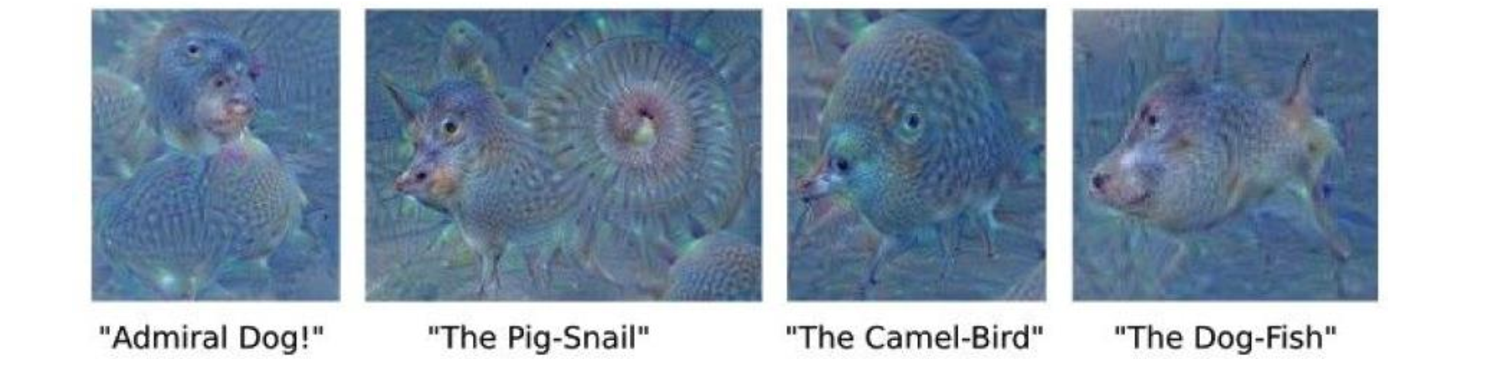
\includegraphics[width=\textwidth]{figures/deepdream2.pdf}
\end{center}
\end{frame}

\begin{frame}{Deep dream}
\begin{center}
  \hspace{-1em}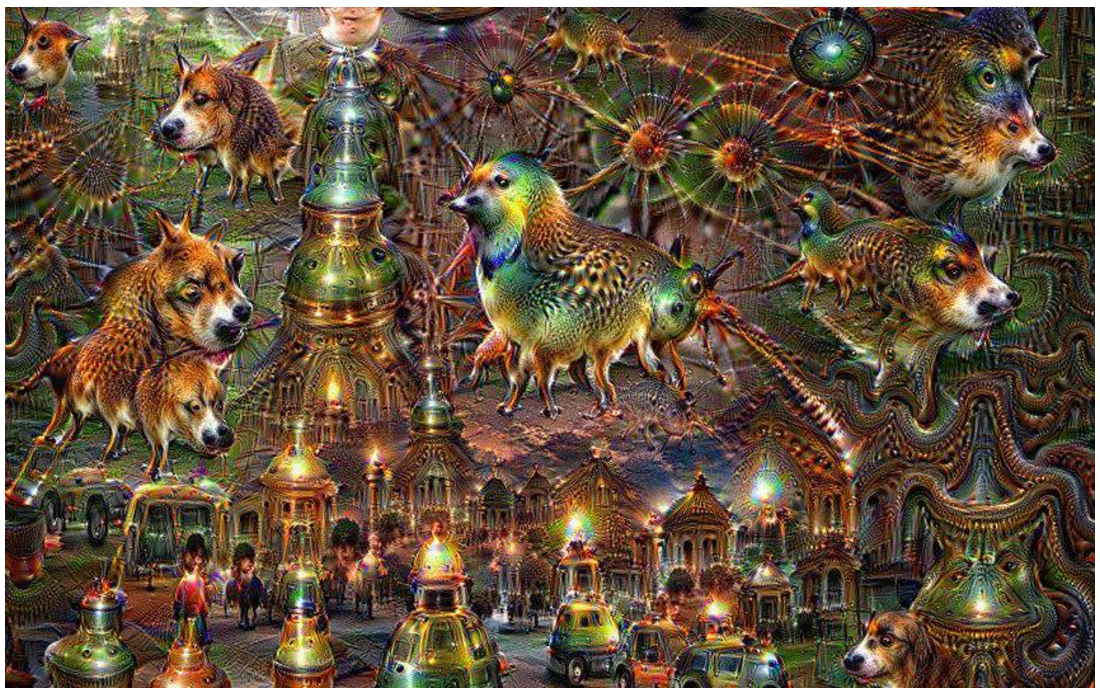
\includegraphics[width=0.9\textwidth]{figures/deepdream3.pdf}
\end{center}
\end{frame}

\begin{frame}{Artistic style transfer}
\begin{itemize}
\item Activation stores content information
\item Activation correlation across space stores style information and discards spatial arrangement
\end{itemize}
\begin{center}
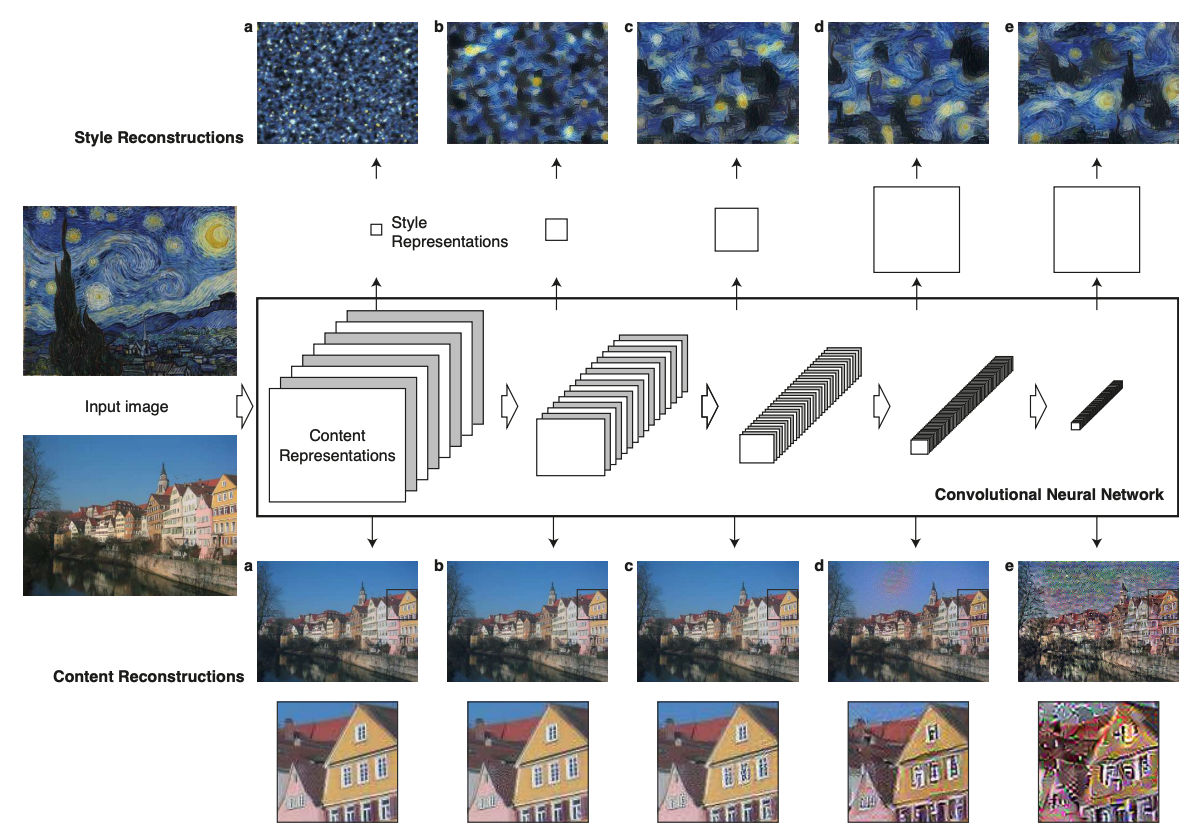
\includegraphics[width=0.55\textwidth]{figures/style_transfer.png}
\end{center}
\begin{flushright}
{\tiny Gatys et al., Image style transfer Using convolutional neural networks, CVPR 2016.}
\end{flushright}

\notenew{
  \begin{itemize}
    \item Backprop into the inputs can generate a lot of interesting patterns.
    \item This could include low level image patterns.
    \item What about change the style of an image?
  \end{itemize}
}
\end{frame}

\begin{frame}{Artistic style transfer}
\begin{itemize}
  \item Optimizing both content \& style from random noise
\end{itemize}
\begin{center}
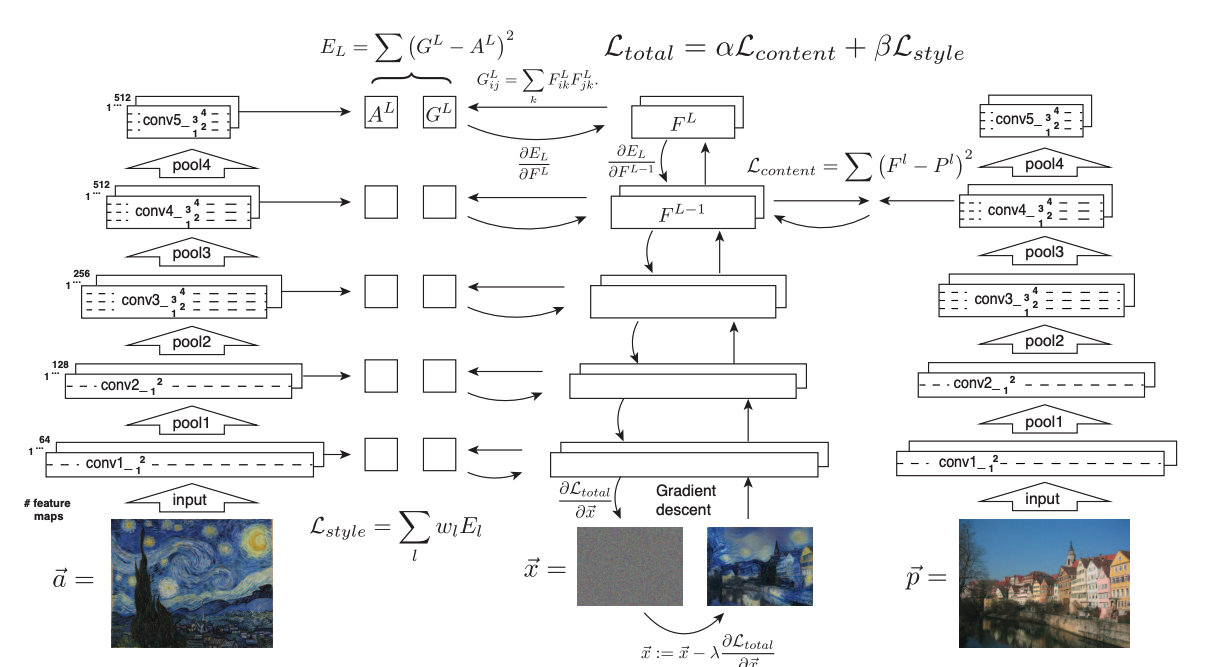
\includegraphics[width=0.85\textwidth]{figures/style_transfer2.png}
\end{center}
\begin{flushright}
{\tiny Gatys et al., Image style transfer Using convolutional neural networks, CVPR 2016.}
\end{flushright}
\end{frame}

\begin{frame}{Artistic style transfer}
\begin{center}
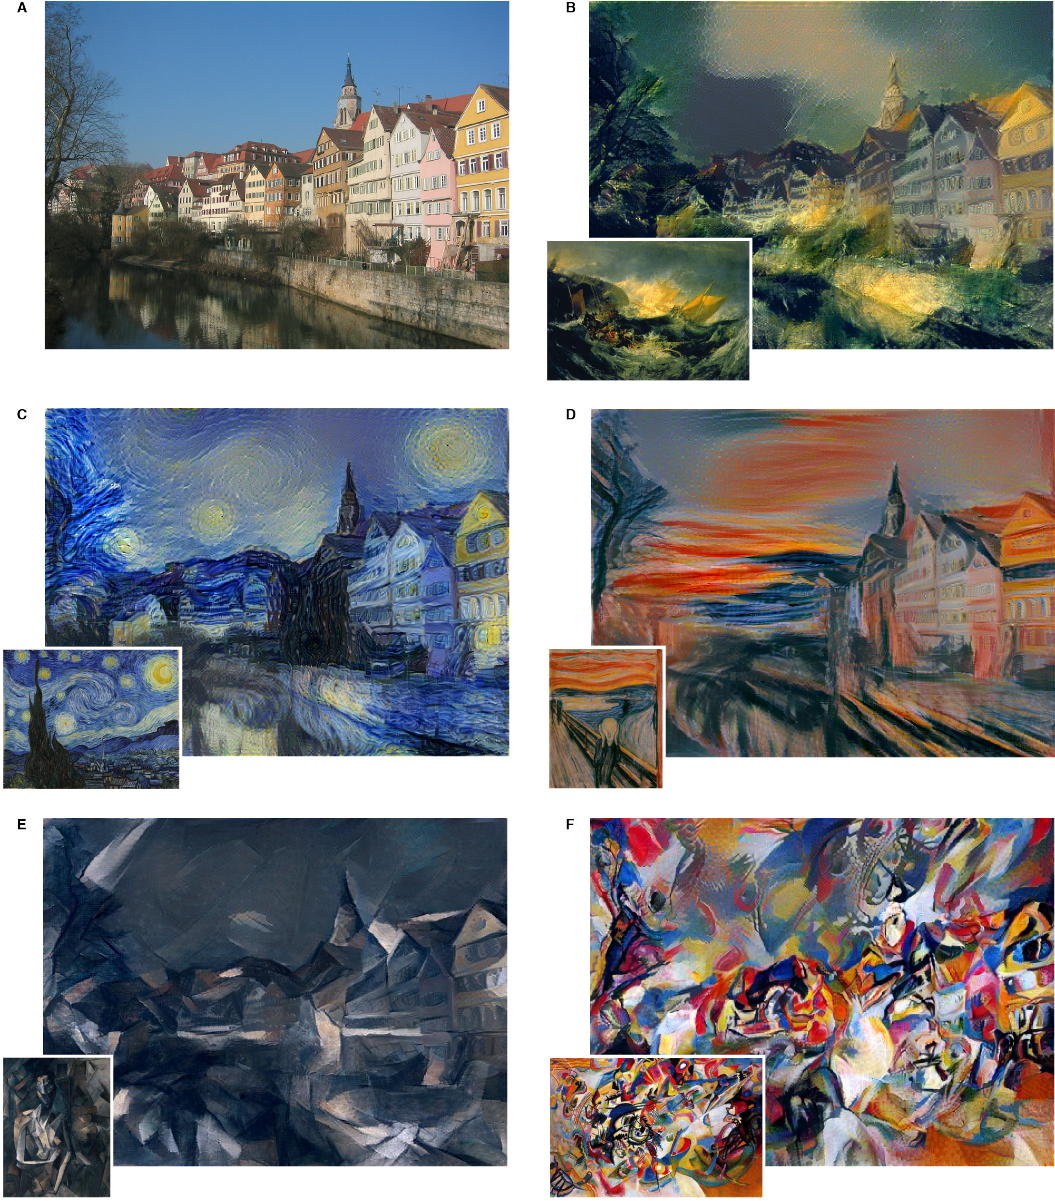
\includegraphics[width=0.7\textwidth,trim={0 7cm 0 0},clip]{figures/style_transfer3.png}
\end{center}
\begin{flushright}
{\tiny Gatys et al., Image style transfer Using convolutional neural networks, CVPR 2016.}
\end{flushright}
\end{frame}

\begin{frame}{Adversarial Examples}
\begin{itemize}
\item One of the most surprising findings about neural nets has been the existence of \high{adversarial inputs}, i.e.~inputs optimized to fool an algorithm.
\end{itemize}
\begin{center}
    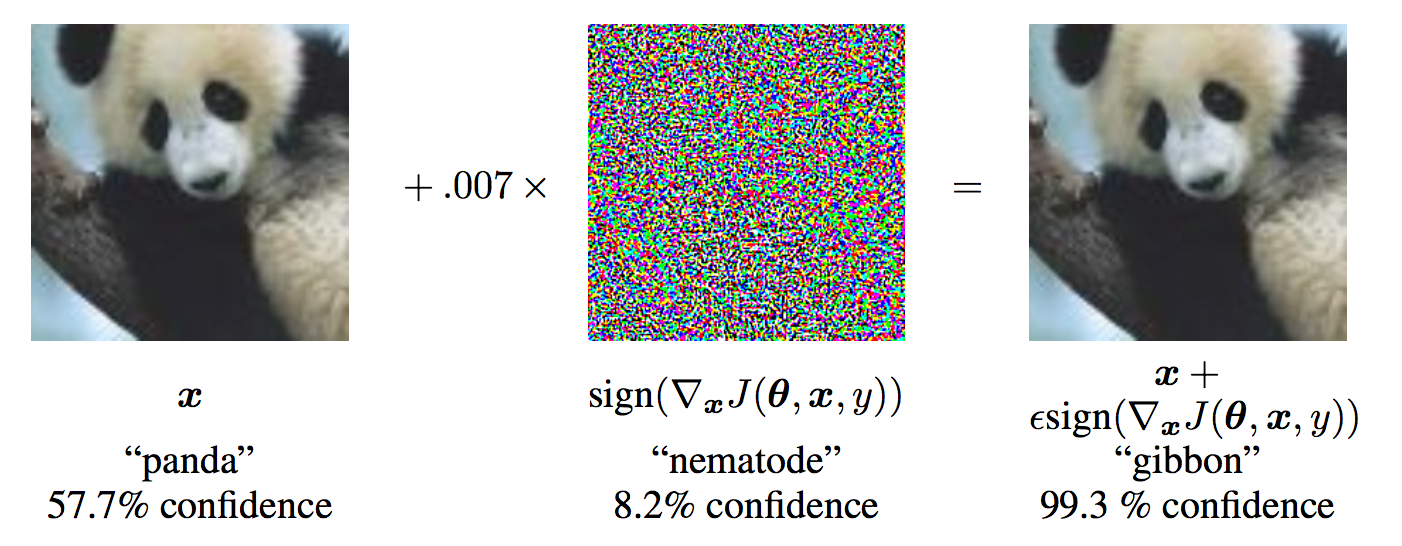
\includegraphics[width=0.75 \linewidth]{figures/fgsm.png}
  \end{center}
\begin{flushright}
  \tiny{Goodfellow et al., Explaining and harnessing adversarial examples, ICLR 2015.}
\end{flushright}
\notenew{
    Given an image for one category (e.g.~``cat''), compute the image gradient to maximize the network's output unit for a different category (e.g.~``dog'')
    \begin{itemize}
      \item Perturb the image very slightly in this direction
      \item Works slightly better if you take the sign of the entries in the gradient; this is called the \high{fast gradient sign method}.
    \end{itemize}
}
\end{frame}

\begin{frame}{Adversarial Examples}
\begin{itemize}
\item The following adversarial examples are misclassified as ostriches. ( $10 \times$ perturbation visualized in middle.)
  \begin{center}
    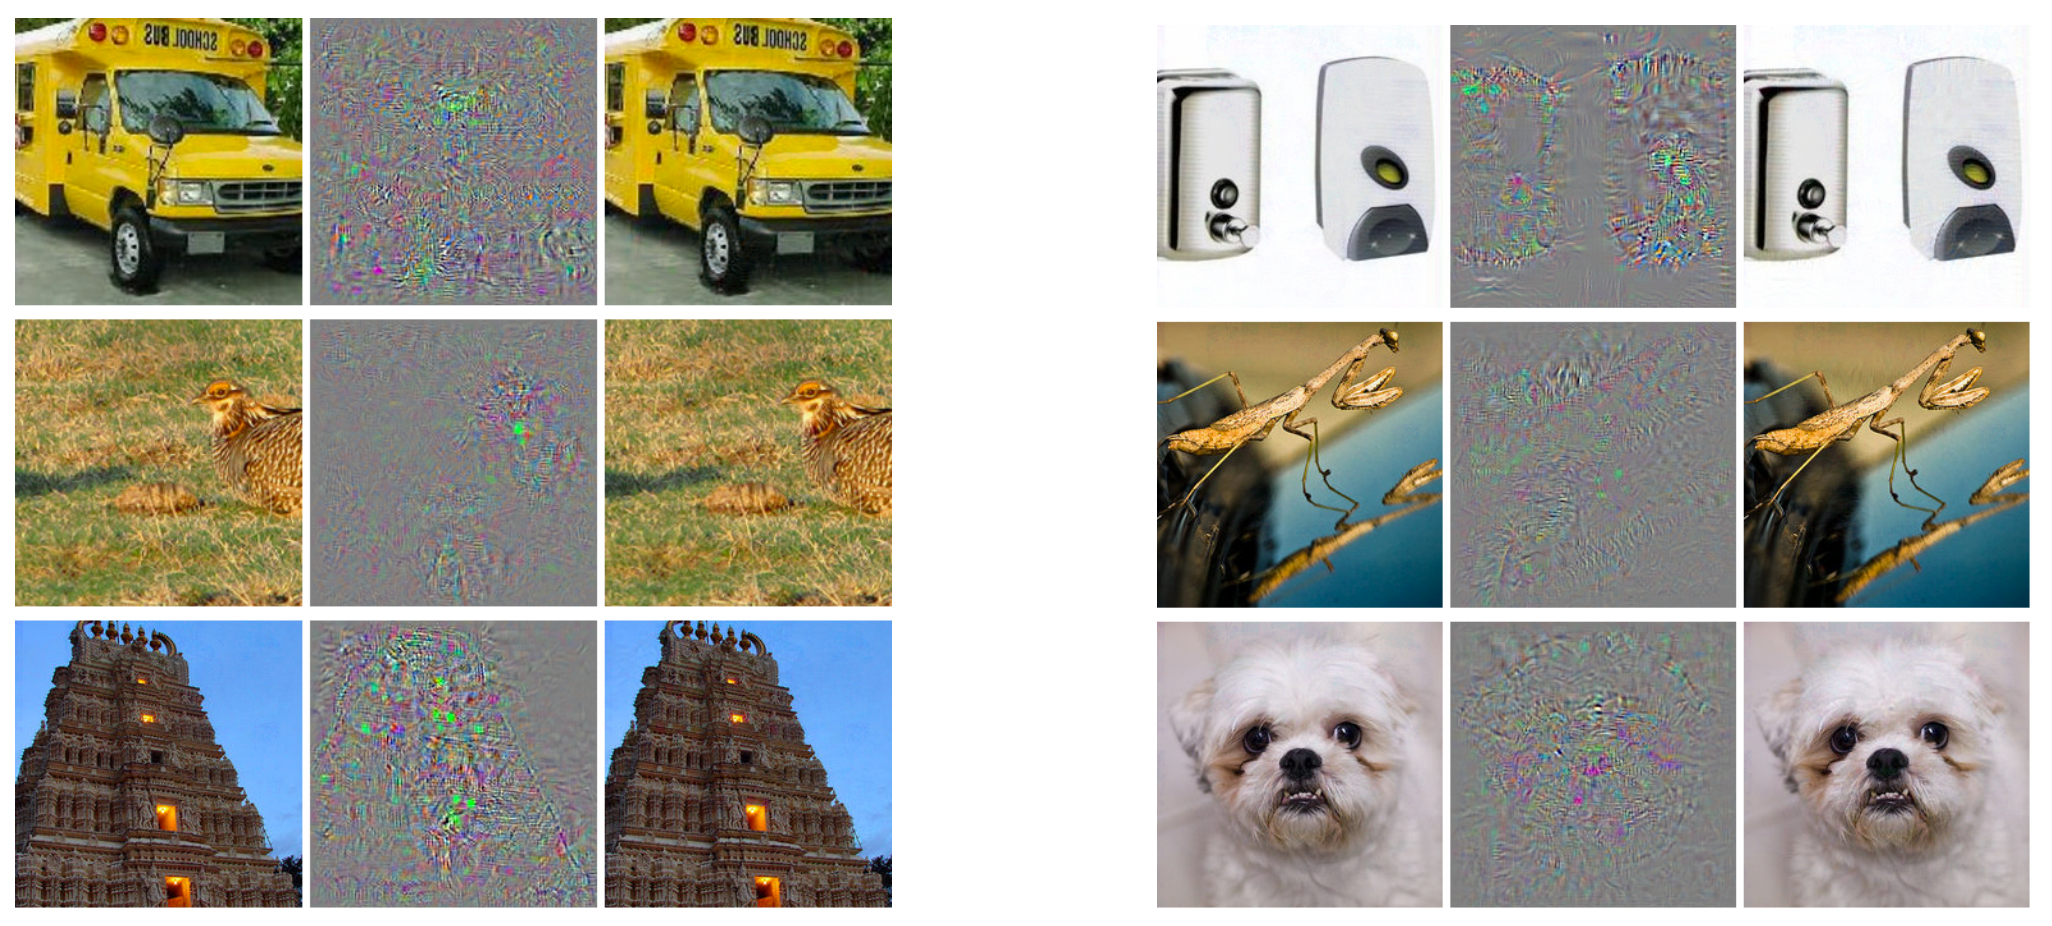
\includegraphics[width=0.85 \linewidth]{figures/adversarial_examples.png}
  \end{center}
\end{itemize}
\begin{flushright}
  \tiny{Szegedy et al., Intriguing properties of neural networks, ICLR 2014.}
\end{flushright}
\end{frame}

\begin{frame}{Adversarial Examples}
\begin{itemize}
\item You can print out an adversarial image and take a picture of it, and it still works!
  \begin{center}
    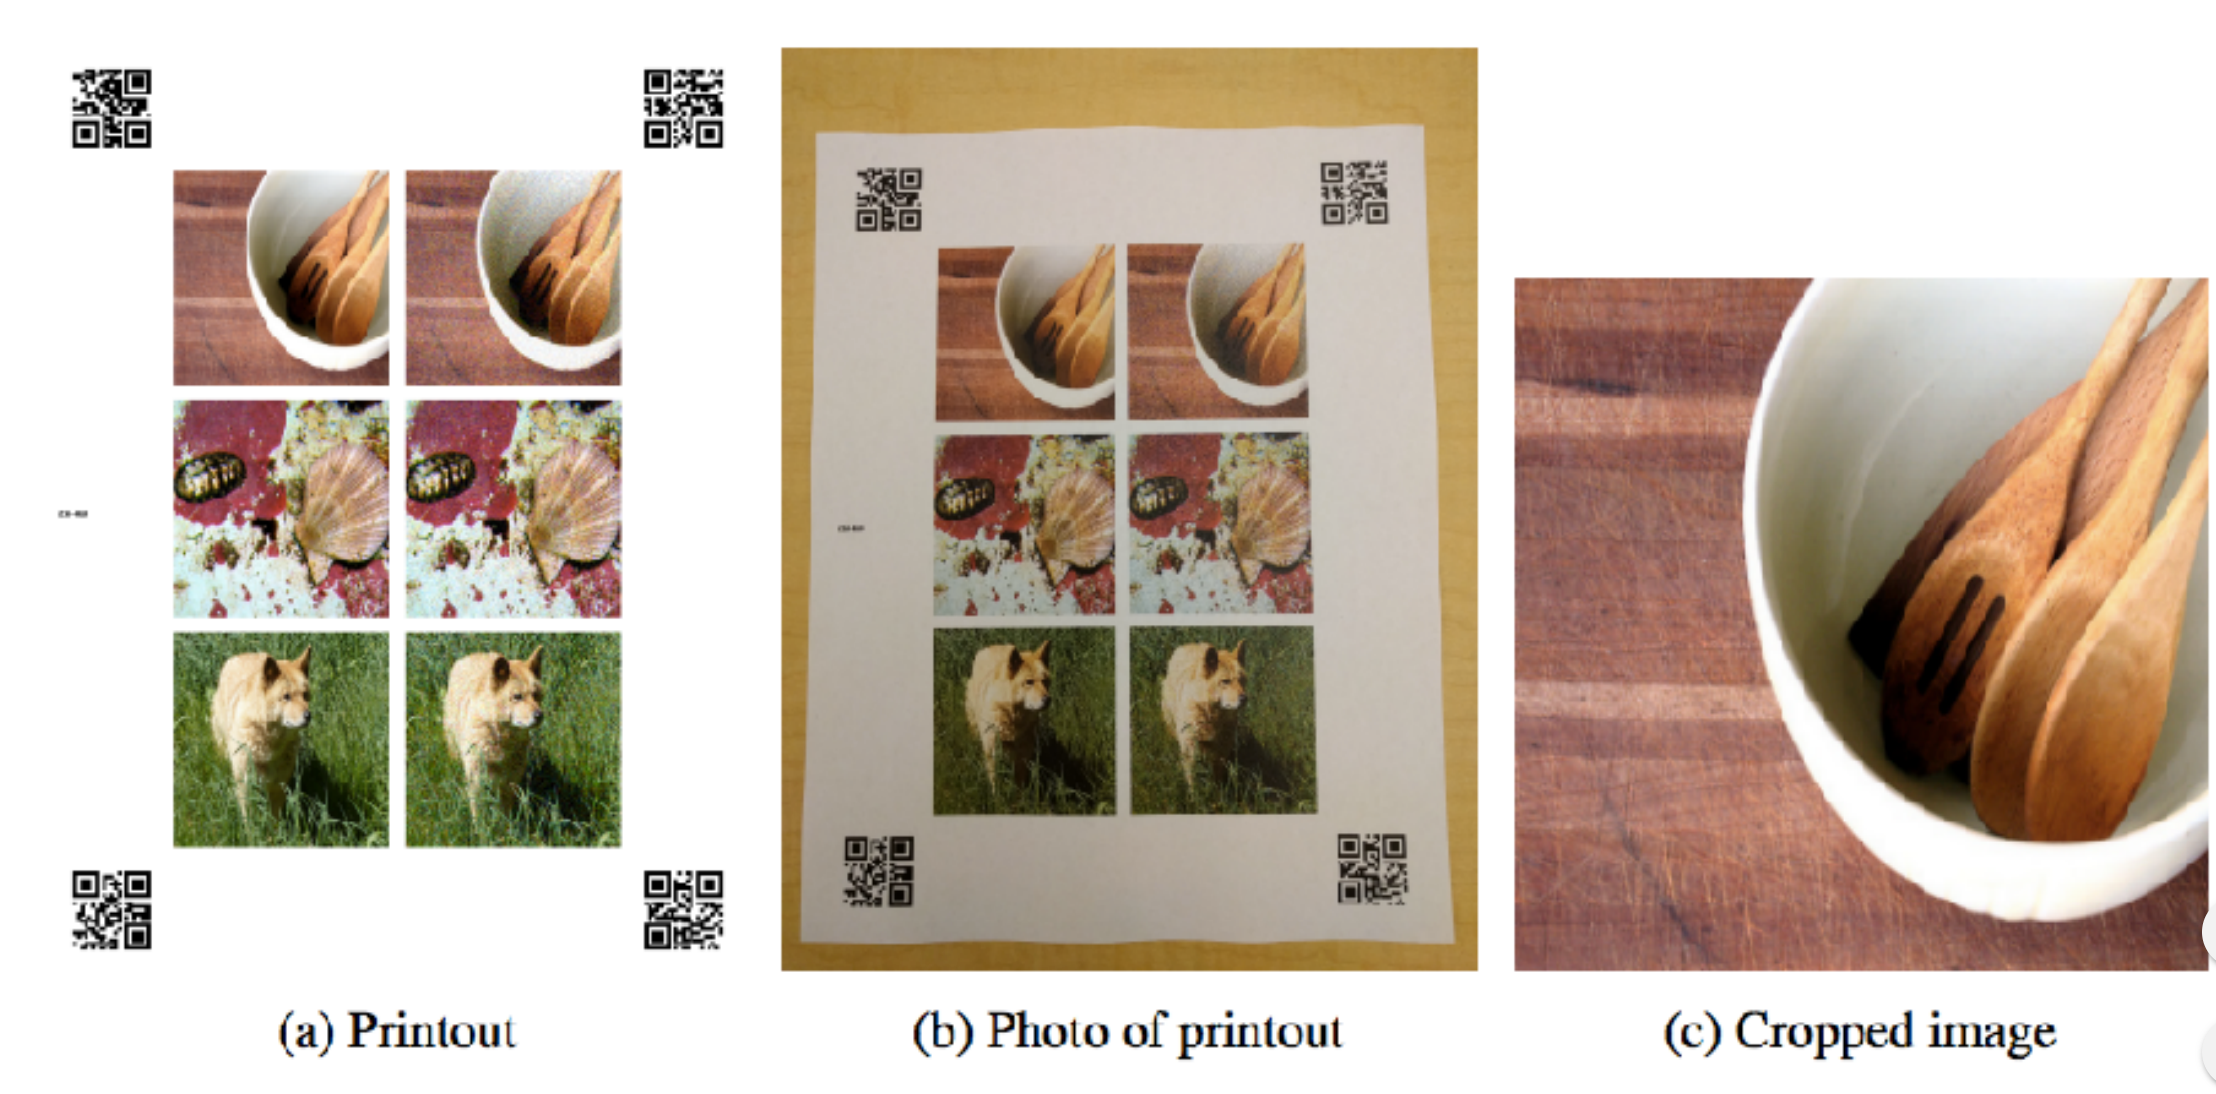
\includegraphics[width=0.9 \linewidth]{figures/printed_adversarial.png}
  \end{center}
  \begin{flushright}
    \tiny{Kurakin et al., Adversarial examples in the physical world, ICLR workshop 2017.}
  \end{flushright}
\end{itemize}
\end{frame}

\begin{frame}{Adversarial Examples}
\begin{itemize}
\item An adversarial example in the physical world (network thinks it's a gun, from a variety of viewing angles!)
  \begin{center}
    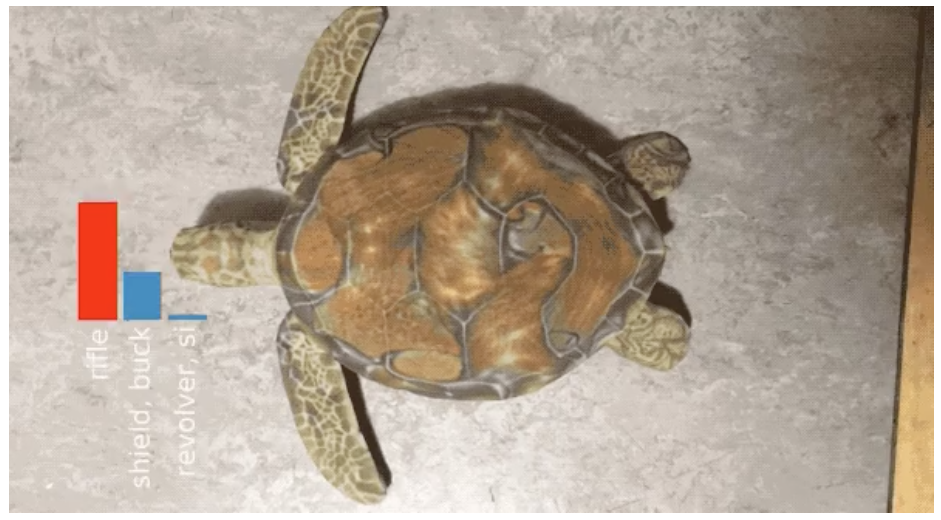
\includegraphics[width=0.8\textwidth]{figures/adversarial_physical.png}
  \end{center}
\end{itemize}
\begin{flushright}
  \tiny{Athalye et al., Synthesizing robust adversarial examples, ICML 2018.}
\end{flushright}
\notenew{
  \begin{itemize}
  \item Optimize different view angles in 3D simulation, randomizing a lot of transformations.
  \end{itemize}
}
\end{frame}

\begin{frame}{Adversarial Examples}
\begin{itemize}
\item An adversarial mesh object that can hide cars from LiDAR detector
  \begin{center}
    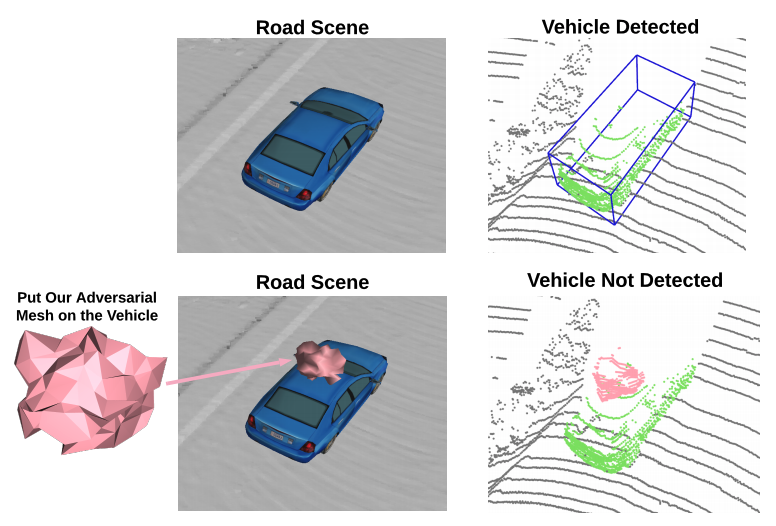
\includegraphics[width=0.6\textwidth]{figures/adv_mesh.png}
  \end{center}
\end{itemize}
\begin{flushright}
  \tiny{Tu et al., Physically realizable adversarial examples for LiDAR object detection, CVPR 2020.}
\end{flushright}
\notenew{
  \begin{itemize}
    \item People often use self-driving car as an example to emphasize the importance.
    \item In this example, this is a 3D vision task, but the intuition is similar.
    \item Tries to fool an object detector with a strange looking shape.
  \end{itemize}
}
\end{frame}


\begin{frame}{Adversarial Defense}
\begin{itemize}
  \item How to defend from adversarial perturbation is still an active research area.
  \item One common approach is to train with millions of adversarial examples.
  \item Needs to train much longer, and also suffers a little from normal accuracy.
\end{itemize}
\notenew{
  More to be covered in security \& privacy of deep learning.
}
\end{frame}


\end{document}
